\let\negmedspace\undefined
\let\negthickspace\undefined
%\RequirePackage{amsmath}
\documentclass[journal,12pt,twocolumn]{IEEEtran}
%
% \usepackage{setspace}
 \usepackage{gensymb}
%\doublespacing
%\singlespacing
%\usepackage{silence}
%Disable all warnings issued by latex starting with "You have..."
%\usepackage{graphicx}
\usepackage{amssymb}
%\usepackage{relsize}
\usepackage[cmex10]{amsmath}
%\usepackage{amsthm}
%\interdisplaylinepenalty=2500
%\savesymbol{iint}
%\usepackage{txfonts}
%\restoresymbol{TXF}{iint}
%\usepackage{wasysym}
\usepackage{amsthm}
%\usepackage{pifont}
%\usepackage{iithtlc}
% \usepackage{mathrsfs}
% \usepackage{txfonts}
 \usepackage{stfloats}
% \usepackage{steinmetz}
 \usepackage{bm}
% \usepackage{cite}
% \usepackage{cases}
% \usepackage{subfig}
%\usepackage{xtab}
\usepackage{longtable}
%\usepackage{multirow}
%\usepackage{algorithm}
%\usepackage{algpseudocode}
\usepackage{enumitem}
 \usepackage{mathtools}
 \usepackage{tikz}
% \usepackage{circuitikz}
% \usepackage{verbatim}
%\usepackage{tfrupee}
\usepackage[breaklinks=true]{hyperref}
%\usepackage{stmaryrd}
%\usepackage{tkz-euclide} % loads  TikZ and tkz-base
%\usetkzobj{all}
\usepackage{listings}
    \usepackage{color}                                            %%
    \usepackage{array}                                            %%
    \usepackage{longtable}                                        %%
    \usepackage{calc}                                             %%
    \usepackage{multirow}                                         %%
    \usepackage{hhline}                                           %%
    \usepackage{ifthen}                                           %%
  %optionally (for landscape tables embedded in another document): %%
    \usepackage{lscape}     
% \usepackage{multicol}
% \usepackage{chngcntr}
%\usepackage{enumerate}

%\usepackage{wasysym}
%\newcounter{MYtempeqncnt}
\DeclareMathOperator*{\Res}{Res}
\DeclareMathOperator*{\equals}{=}
%\renewcommand{\baselinestretch}{2}
\renewcommand\thesection{\arabic{section}}
\renewcommand\thesubsection{\thesection.\arabic{subsection}}
\renewcommand\thesubsubsection{\thesubsection.\arabic{subsubsection}}

\renewcommand\thesectiondis{\arabic{section}}
\renewcommand\thesubsectiondis{\thesectiondis.\arabic{subsection}}
\renewcommand\thesubsubsectiondis{\thesubsectiondis.\arabic{subsubsection}}

% correct bad hyphenation here
\hyphenation{op-tical net-works semi-conduc-tor}
\def\inputGnumericTable{}                                 %%

\lstset{
%language=C,
frame=single, 
breaklines=true,
columns=fullflexible
}
%\lstset{
%language=tex,
%frame=single, 
%breaklines=true
%}
\begin{document}

%


\newtheorem{theorem}{Theorem}[section]
\newtheorem{problem}{Problem}
\newtheorem{proposition}{Proposition}[section]
\newtheorem{lemma}{Lemma}[section]
\newtheorem{corollary}[theorem]{Corollary}
\newtheorem{example}{Example}[section]
\newtheorem{definition}[problem]{Definition}
%\newtheorem{thm}{Theorem}[section] 
%\newtheorem{defn}[thm]{Definition}
%\newtheorem{algorithm}{Algorithm}[section]
%\newtheorem{cor}{Corollary}
\newcommand{\BEQA}{\begin{eqnarray}}
\newcommand{\EEQA}{\end{eqnarray}}
\newcommand{\define}{\stackrel{\triangle}{=}}
\newcommand*\circled[1]{\tikz[baseline=(char.base)]{
    \node[shape=circle,draw,inner sep=2pt] (char) {#1};}}
\bibliographystyle{IEEEtran}
%\bibliographystyle{ieeetr}


\providecommand{\mbf}{\mathbf}
\providecommand{\pr}[1]{\ensuremath{\Pr\left(#1\right)}}
\providecommand{\qfunc}[1]{\ensuremath{Q\left(#1\right)}}
\providecommand{\sbrak}[1]{\ensuremath{{}\left[#1\right]}}
\providecommand{\lsbrak}[1]{\ensuremath{{}\left[#1\right.}}
\providecommand{\rsbrak}[1]{\ensuremath{{}\left.#1\right]}}
\providecommand{\brak}[1]{\ensuremath{\left(#1\right)}}
\providecommand{\lbrak}[1]{\ensuremath{\left(#1\right.}}
\providecommand{\rbrak}[1]{\ensuremath{\left.#1\right)}}
\providecommand{\cbrak}[1]{\ensuremath{\left\{#1\right\}}}
\providecommand{\lcbrak}[1]{\ensuremath{\left\{#1\right.}}
\providecommand{\rcbrak}[1]{\ensuremath{\left.#1\right\}}}
\theoremstyle{remark}
\newtheorem{rem}{Remark}
\newcommand{\sgn}{\mathop{\mathrm{sgn}}}
\providecommand{\abs}[1]{\left\vert#1\right\vert}
\providecommand{\res}[1]{\Res\displaylimits_{#1}} 
\providecommand{\norm}[1]{\left\lVert#1\right\rVert}
%\providecommand{\norm}[1]{\lVert#1\rVert}
\providecommand{\mtx}[1]{\mathbf{#1}}
\providecommand{\mean}[1]{E\left[ #1 \right]}
\providecommand{\fourier}{\overset{\mathcal{F}}{ \rightleftharpoons}}
%\providecommand{\hilbert}{\overset{\mathcal{H}}{ \rightleftharpoons}}
\providecommand{\system}{\overset{\mathcal{H}}{ \longleftrightarrow}}
	%\newcommand{\solution}[2]{\textbf{Solution:}{#1}}
\newcommand{\solution}{\noindent \textbf{Solution: }}
\newcommand{\cosec}{\,\text{cosec}\,}
\providecommand{\dec}[2]{\ensuremath{\overset{#1}{\underset{#2}{\gtrless}}}}
\newcommand{\myvec}[1]{\ensuremath{\begin{pmatrix}#1\end{pmatrix}}}
\newcommand{\mydet}[1]{\ensuremath{\begin{vmatrix}#1\end{vmatrix}}}
%\numberwithin{equation}{section}
\numberwithin{equation}{subsection}
%\numberwithin{problem}{section}
%\numberwithin{definition}{section}
\makeatletter
\@addtoreset{figure}{problem}
\makeatother

\let\StandardTheFigure\thefigure
\let\vec\mathbf
%\renewcommand{\thefigure}{\theproblem.\arabic{figure}}
\renewcommand{\thefigure}{\theproblem}
%\setlist[enumerate,1]{before=\renewcommand\theequation{\theenumi.\arabic{equation}}
%\counterwithin{equation}{enumi}


%\renewcommand{\theequation}{\arabic{subsection}.\arabic{equation}}

\def\putbox#1#2#3{\makebox[0in][l]{\makebox[#1][l]{}\raisebox{\baselineskip}[0in][0in]{\raisebox{#2}[0in][0in]{#3}}}}
     \def\rightbox#1{\makebox[0in][r]{#1}}
     \def\centbox#1{\makebox[0in]{#1}}
     \def\topbox#1{\raisebox{-\baselineskip}[0in][0in]{#1}}
     \def\midbox#1{\raisebox{-0.5\baselineskip}[0in][0in]{#1}}

\vspace{3cm}

\title{
	%\logo{
%Computational Approach to School Geometry
	Matrix Analysis
%	}
}
\author{ G V V Sharma$^{*}$% <-this % stops a space
	\thanks{*The author is with the Department
		of Electrical Engineering, Indian Institute of Technology, Hyderabad
		502285 India e-mail:  gadepall@iith.ac.in. All content in this manual is released under GNU GPL.  Free and open source.}
	
}	
%\title{
%	\logo{Matrix Analysis through Octave}{\begin{center}\includegraphics[scale=.24]{tlc}\end{center}}{}{HAMDSP}
%}


% paper title
% can use linebreaks \\ within to get better formatting as desired
%\title{Matrix Analysis through Octave}
%
%
% author names and IEEE memberships
% note positions of commas and nonbreaking spaces ( ~ ) LaTeX will not break
% a structure at a ~ so this keeps an author's name from being broken across
% two lines.
% use \thanks{} to gain access to the first footnote area
% a separate \thanks must be used for each paragraph as LaTeX2e's \thanks
% was not built to handle multiple paragraphs
%

%\author{<-this % stops a space
%\thanks{}}
%}
% note the % following the last \IEEEmembership and also \thanks - 
% these prevent an unwanted space from occurring between the last author name
% and the end of the author line. i.e., if you had this:
% 
% \author{....lastname \thanks{...} \thanks{...} }
%                     ^------------^------------^----Do not want these spaces!
%
% a space would be appended to the last name and could cause every name on that
% line to be shifted left slightly. This is one of those "LaTeX things". For
% instance, "\textbf{A} \textbf{B}" will typeset as "A B" not "AB". To get
% "AB" then you have to do: "\textbf{A}\textbf{B}"
% \thanks is no different in this regard, so shield the last } of each \thanks
% that ends a line with a % and do not let a space in before the next \thanks.
% Spaces after \IEEEmembership other than the last one are OK (and needed) as
% you are supposed to have spaces between the names. For what it is worth,
% this is a minor point as most people would not even notice if the said evil
% space somehow managed to creep in.

%\WarningFilter{latex}{LaTeX Warning: You have requested, on input line 117, version}


% The paper headers
%\markboth{Journal of \LaTeX\ Class Files,~Vol.~6, No.~1, January~2007}%
%{Shell \MakeLowercase{\textit{et al.}}: Bare Demo of IEEEtran.cls for Journals}
% The only time the second header will appear is for the odd numbered pages
% after the title page when using the twoside option.
% 
% *** Note that you probably will NOT want to include the author's ***
% *** name in the headers of peer review papers.                   ***
% You can use \ifCLASSOPTIONpeerreview for conditional compilation here if
% you desire.




% If you want to put a publisher's ID mark on the page you can do it like
% this:
%\IEEEpubid{0000--0000/00\$00.00~\copyright~2007 IEEE}
% Remember, if you use this you must call \IEEEpubidadjcol in the second
% column for its text to clear the IEEEpubid mark.



% make the title area
\maketitle

\newpage

\tableofcontents

\bigskip

\renewcommand{\thefigure}{\theenumi}
\renewcommand{\thetable}{\theenumi}
%\renewcommand{\theequation}{\theenumi}

%\begin{abstract}
%%\boldmath
%In this letter, an algorithm for evaluating the exact analytical bit error rate  (BER)  for the piecewise linear (PL) combiner for  multiple relays is presented. Previous results were available only for upto three relays. The algorithm is unique in the sense that  the actual mathematical expressions, that are prohibitively large, need not be explicitly obtained. The diversity gain due to multiple relays is shown through plots of the analytical BER, well supported by simulations. 
%
%\end{abstract}
% IEEEtran.cls defaults to using nonbold math in the Abstract.
% This preserves the distinction between vectors and scalars. However,
% if the journal you are submitting to favors bold math in the abstract,
% then you can use LaTeX's standard command \boldmath at the very start
% of the abstract to achieve this. Many IEEE journals frown on math
% in the abstract anyway.

% Note that keywords are not normally used for peerreview papers.
%\begin{IEEEkeywords}
%Cooperative diversity, decode and forward, piecewise linear
%\end{IEEEkeywords}



% For peer review papers, you can put extra information on the cover
% page as needed:
% \ifCLASSOPTIONpeerreview
% \begin{center} \bfseries EDICS Category: 3-BBND \end{center}
% \fi
%
% For peerreview papers, this IEEEtran command inserts a page break and
% creates the second title. It will be ignored for other modes.
%\IEEEpeerreviewmaketitle

\begin{abstract}
This manual provides an introduction to vectors and their properties,  based on the question papers, year 2020,  from Class 10 and 12, CBSE; JEE and JNTU.  
\end{abstract}

\section{Class 10}
\renewcommand{\theequation}{\theenumi}
%\begin{enumerate}[label=\arabic*.,ref=\theenumi]
\begin{enumerate}[label=\thesection.\arabic*.,ref=\thesection.\theenumi]
\numberwithin{equation}{enumi}
\item  Find the distance between the points $\myvec{m \\ -n}$ and $\myvec{-m \\ n}$
	\\
		\solution Letting 
		\begin{align}
			\vec{A} &= \myvec{m \\ -n}, \vec{B}=\myvec{-m \\ n}
			\\
			\vec{A}-\vec{B} &= 2\myvec{m \\ -n}
			\\
			\implies \norm{\vec{A}-\vec{B}} &=2\norm{\myvec{m \\ -n}}
			\\
			&=2 \sqrt{\myvec{m & -n}\myvec{m \\ -n}} 
\\
			&			= 2 \sqrt{m^2+n^2}
		\end{align}
	\item Find a point on the $x-$axis which is equidistant from $\myvec{ -4 \\ 0}$ and $\myvec{10 \\ 0}$
\\
\solution Letting the given points be $\vec{A},\vec{B}$. 

\begin{enumerate}

	\item 
		\begin{align}
	\because  \vec{A}-\vec{B} &= \myvec{ -4 \\ 0}-\myvec{10 \\ 0}
	  \\
	  &= \myvec{ -14 \\ 0},
	  \\
			\text{and }	   \frac{\norm{\vec{A}}^2 - \norm{\vec{B}}^2}{2} &= -42,
  \end{align}
  \eqref{eq:norm2d_equidist}, can be expressed as 
  \begin{align}
	  \myvec{ -14 & 0}\vec{x} 
	  &=  42
	  \\
	  \implies 
	  \myvec{ -14 & 0}\myvec{x \\ 0} 
	  &=  -42
	  \\
	  \text{or, } x =3 
  \end{align}
  Hence, the desired point is $\myvec{ 3 \\ 0}$.
\item In general, if $\vec{x}$ be the desired point, 
  \begin{align}
	  \norm{\vec{x}-\vec{A}}
	  &=
	  \norm{\vec{x}-\vec{B}}
	  \\
	  \implies \norm{\vec{x}-\vec{A}}^2
	  &=
	  \norm{\vec{x}-\vec{B}}^2
  \end{align}
  which can be expressed as 
  \begin{multline}
	  \norm{\vec{x}}^2+\norm{\vec{A}}^2 - 2 \vec{A}^{\top }\vec{x}
	  \\
	  =
	  \norm{\vec{x}}^2+\norm{\vec{B}}^2 - 2 \vec{B}^{\top }\vec{x}
  \end{multline}
  and simplified to obtain 
  \begin{align}
	  \label{eq:cbse_10_x}
	   \brak{\vec{A}-\vec{B}}^{\top }\vec{x}
	  =
	  \frac{\norm{\vec{A}}^2 -\norm{\vec{B}}^2 }{2}
  \end{align}
  Since $\vec{x}$ lies on the $x$-axis, 
  \begin{align}
	  \vec{x} &=
	   x\vec{e}_1
	  \\
	  \implies 
	   x\brak{\vec{A}-\vec{B}}^{\top }\vec{e}_1
		  &=
	  \frac{\norm{\vec{A}}^2 -\norm{\vec{B}}^2 }{2}
	  \\
	  \text{or, } x &=\frac{\norm{\vec{A}}^2 -\norm{\vec{B}}^2 }{2\brak{\vec{A}-\vec{B}}^{\top }\vec{e}_1
}
  \end{align}
	  upon substituting from \eqref{eq:cbse_10_x}.


		\begin{align}
	\because  \vec{A}-\vec{B} &= \myvec{ -4 \\ 0}-\myvec{10 \\ 0}
	  \\
	  &= \myvec{ -14 \\ 0},
	  \\
			\text{and }	   \frac{\norm{\vec{A}}^2 - \norm{\vec{B}}^2}{2} &= -42,
  \end{align}
  \eqref{eq:norm2d_equidist}, can be expressed as 
  \begin{align}
	  \myvec{ -14 & 0}\vec{x} 
	  &=  42
	  \\
	  \implies 
	  \myvec{ -14 & 0}\myvec{x \\ 0} 
	  &=  -42
	  \\
	  \text{or, } x =3 
  \end{align}
  Hence, the desired point is $\myvec{ 3 \\ 0}$.
  \end{enumerate}
  \item Find the centre of a circle whose end points of a diameter are $\myvec{ -6 \\ 3}$ and $\myvec{6 \\ 4}$.
	  \\
		\solution 
Using section formula, 
	  from \eqref{eq:section_formula},
		the desired point is given by 
  \begin{align}
	  \vec{O}&= \frac{\vec{B}+ \vec{A}}{2}
	  \\
	  &= \frac{1}{2}\sbrak{\myvec{ -6 \\ 3}+\myvec{6 \\ 4}}
	  \\
	  &=\frac{1}{2}\myvec{0 \\ 7}
  \end{align}
    See Fig. 
	  \ref{fig:cbse-10-3.pdf}
  \begin{figure}
	  \centering 
	  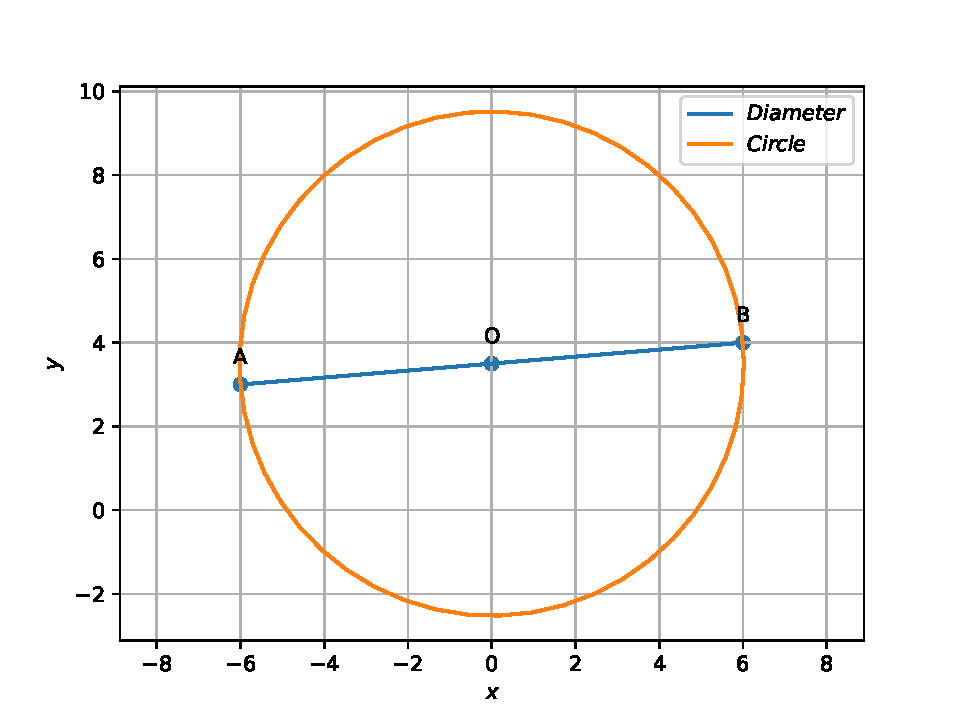
\includegraphics[width=\columnwidth]{figs/cbse-10-3.pdf}
	  \caption{}
	  \label{fig:cbse-10-3.pdf}
	  \end{figure}

  \item $AOBC$  is a rectangle whose three vertices are $A = \myvec{0\\-3}, O = \myvec{0\\0}, B = \myvec{4\\0}$.  Find the length of its diagonal. 
	  \\
		\solution 
\begin{enumerate}
	\item The fourth point is given by 
  \begin{align}
	 OC =  \vec{C}&=\myvec{4 \\ -3}
  \end{align}
  The length of the diagonal is 
		\begin{align}
			\norm{\vec{C}} &= 
			 \sqrt{\myvec{4 & -3}\myvec{4 \\ -3}} 
\\
			&			=  \sqrt{25} = 5
		\end{align}
	\item  In general, if three vertices of a rectangle are given, the adjacent sides need to be identified first to identify the opposite vertices.  For example, in the given problem,  
  \begin{align}
	  \brak{\vec{A}-\vec{O}}^{\top}\brak{\vec{B}-\vec{O}} &= 0	 
	  \\
	  \implies \angle AOB &= 90\degree
  \end{align}
  and $AB$ is the diagonal.
This condition needs to be checked before proceeding to find the length of the diagonal.
\end{enumerate}
	\item  Find the ratio in which the $y$-axis divides the line segment joining the points $\myvec{6 \\ -4}, \myvec{-2 \\ -7} $.  Also find the point of intersection.
		\\
		\solution  Let the desired point on the $y$-axis be  
		\begin{align}
\vec{P} = \myvec{0 \\ y}
		\end{align}
		\begin{enumerate}
		\item Using section formula, 
	  from \eqref{eq:section_formula},
		\begin{align}
			\vec{P} &= \myvec{0 \\ y}= \frac{1}{k+1}\sbrak{\myvec{6 \\ -4}+ k\myvec{-2 \\ -7} }
			\\
			&	\implies 6 - 2k = 0 \text{ or, }k = 3
		\end{align}
		Also, 
		\begin{align}
			y &= \frac{-4-7k}{k+1}
			\\
			&=-\frac{25}{4}
		\end{align}
		Thus, the desired point is  $ -\frac{25}{4}
\myvec{0 \\ 1 }$.
\item In general, letting the given points be $\vec{A}, \vec{B}$, 
		\begin{align}
			\vec{P} &= \frac{k\vec{B}+ \vec{A} }{k+1}
			\label{eq:cbse-10-5-section}
		\end{align}
		Since the point lies on the $y$-axis, 
		\begin{align}
			\vec{e}_1^{\top}\vec{P} &= 0
			\\
			\implies k\vec{e}_1^{\top}\vec{B}+ \vec{e}_1^{\top}\vec{A} &=0
			\\
			\text{or, } k &=- \frac{\vec{e}_1^{\top}\vec{A}}{\vec{e}_1^{\top}\vec{B}}
		\end{align}
Substituting in 			\eqref{eq:cbse-10-5-section} and simplifying, 
		\begin{align}
			\vec{P} &= \frac{\brak{\vec{e}_1^{\top}\vec{B}}\vec{A}- \brak{\vec{e}_1^{\top}\vec{A}}\vec{B} }{\brak{\vec{e}_1^{\top}\vec{B}}-\brak{\vec{e}_1^{\top}\vec{A}}}
		\end{align}
		\end{enumerate}
	\item   Show that the points $\myvec{7 \\ 10}, \myvec{-2 \\ 5} $ and $\myvec{3 \\ -4}$ are vertices of an isoscles right triangle.
		\\
		\solution Let the given points be $\vec{A}, \vec{B}, \vec{C}$ respectively. 
		\begin{enumerate}
			\item Then, the direction vectors of $AB, BC$ and $CA$ are
		\begin{align}
			\vec{A} -\vec{B}&= \myvec{7 \\ 10} -\myvec{-2 \\ 5} = \myvec{9 \\ 5}
			\\
			\vec{B} -\vec{C}&=  -\myvec{-2 \\ 5}-\myvec{3 \\ -4} = \myvec{-5 \\ 9}
			\\
			\vec{C} -\vec{A}&= \myvec{3 \\ -4} -\myvec{7 \\ 10} = \myvec{-4 \\ -14}
		\end{align}
		From the above,  we find that 
		\begin{align}
			\brak{\vec{A} -\vec{B}}^{\top}\brak{\vec{B} -\vec{C}}&=  \myvec{9 & 5}\myvec{-5 \\ 9}
			\\
			&=0
			\\
			\brak{\vec{B} -\vec{C}}^{\top}\brak{\vec{C} -\vec{A}}&=  \myvec{-5 & 9}\myvec{-4 \\ -14}
\\
			&=-106
			\\
			\brak{\vec{C} -\vec{A}}^{\top}\brak{\vec{A} -\vec{B}}&=  \myvec{-4 & -14}\myvec{9 \\ 5}
\\
			&=-106
		\end{align}
		From  the above equations, 
    \eqref{eq:angle2d} and 
    \eqref{eq:angle2d_orth},
		\begin{align}
			\brak{\vec{A} -\vec{B}}\perp \brak{\vec{B} -\vec{C}}
			\\
			\angle BCA = 
			\angle CAB  
		\end{align}
		Thus, the triangle is right angled and isosceles.
	\item In general,  for an isosceles triangle, if $AB = BC$,
		\begin{align}
			\angle BCA &= 
			\angle CAB,  
			\\
			\implies \frac{\brak{\vec{C}-\vec{B}}^{\top}\brak{\vec{C}-\vec{A}}}{\norm{\vec{C}-\vec{B}}\norm{\vec{C}-\vec{A}}}
			&=\frac{\brak{\vec{A}-\vec{C}}^{\top}\brak{\vec{A}-\vec{B}}}{\norm{\vec{A}-\vec{C}}\norm{\vec{A}-\vec{B}}}
			\\
			\text{or }\brak{\vec{C}-\vec{B}}^{\top}\brak{\vec{C}-\vec{A}} &= \brak{\vec{A}-\vec{C}}^{\top}\brak{\vec{A}-\vec{B}}
		\end{align}
		The above condition needs to be checked for each pair of sides to determine whether the triangle is isosceles.
		\end{enumerate}
\end{enumerate}
\section{Class 12}
\renewcommand{\theequation}{\theenumi}
%\begin{enumerate}[label=\arabic*.,ref=\theenumi]
\begin{enumerate}[label=\thesection.\arabic*.,ref=\thesection.\theenumi]
\numberwithin{equation}{enumi}
	\item Find the area of a triangle formed by vertices O, A and B, where 
		\begin{align}
			\vec{A} = \myvec{1 \\ 2 \\ 3},
			\vec{B}  = \myvec{-3 \\ -2 \\ 1},
		\end{align}
\solution $\because $
		\begin{align}
			\myvec{2 & -2 \\ 3 & 1 } &= 8,
\\
			\myvec{3 & 1 \\ 1 & -3 } &= -10,
			\\
			\myvec{1 & -3 \\ 2 & -2 } &= 4,
		\end{align}
		\begin{align}
			\vec{A}  \times 
			\vec{B}  = \myvec{8 \\ -10 \\ 4},
		\end{align}
		and the  desired area can be obtained from 
  \eqref{eq:cross3d} and 
  \eqref{eq:area3d} as
		\begin{align}
			\frac{1}{2}\norm{\myvec{8 \\ -10 \\ 4}} = 3 \sqrt{5}
		\end{align}
	\item  Find the coordinates of the foot of the perpendicular drawn from the point $ \myvec{2 \\-3 \\4 } $ on the y-axis.
		\\
\solution By definition of $y$-axis, the desired coordinates are 
		\begin{align}
			\myvec{0 \\ -3 \\ 0} 
		\end{align}
	Alternatively, the equation of the $y$-axis can be written as	
		\begin{align}
			\vec{x} = \lambda 	\myvec{0 \\ 1 \\ 0} 
		\end{align}
		The equation of the plane perpendicular to the $y$-axis and passing through the origin is
		\begin{align}
 	\myvec{0 \\ 1 \\ 0} \vec{x} = 0
		\end{align}
	From \eqref{eq:plane_line_foot_ans},  the desired point is given by 
\begin{align}
	\vec{x} &=   \myvec{0 & 1 & 0}\myvec{2 \\-3 \\4 } 
 \myvec{0 \\ 1 \\ 0} 
 \\
	&=
 \myvec{0 \\ -3 \\ 0} 
		\end{align}
	\item  Find the angle between the vectors $ \myvec{1 \\ -1 \\ 0} $ and $ \myvec{0 \\ 1 \\ -1} $ 
\\
\solution $\because$
%
  \begin{align}
	  \myvec{1 & -1 & 0} \myvec{0 \\ 1 \\ -1} &= -1,
	  \norm{\myvec{1 \\ -1 \\ 0}}=\norm{\myvec{0 \\ 1 \\ -1}} &= \sqrt{2}
  \end{align}
		From 
    \eqref{eq:angle2d}, the angle between the given vectors is 
  \begin{align}
 \cos^{-1}\frac{-1}{\sqrt{2} \times 
\sqrt{2}
	  } &= 
 \cos^{-1}\frac{-1}{2
	  } 
	  \\
	  &= \frac{2\pi}{3}
  \end{align}
\item  If A is a non-singular square matrix of order 3 such that $ \vec{A}^2 =3\vec{ A}$, then find the value of  $\mydet{\vec{A}}$ 
	\\
	\solution 
  \begin{align}
	  \mydet {\vec{A}^2} &=\mydet{3\vec{ A}}
	  \\
	  \implies 
	  \mydet {\vec{A}} ^2&=3^3\mydet{\vec{ A}}
  \end{align}
  from 
	\eqref{eq:det_kord}
	yielding 
  \begin{align}
	  \mydet {\vec{A}} &=27
  \end{align}
  after simplification.
\item  If $\norm{\vec{a}}
	 = 4 $ and  $ -3\leq \lambda \leq 2 $ then find the range of values that $\norm{\lambda \vec{a}}$ can satisfy.
	 \\
	 \solution  From 
  \eqref{eq:norm2d_const}, 
\begin{align}
  \norm{\lambda \vec{a}} 
  &= \abs{\lambda} \norm{\vec{A}}
  \\
	&= 4\abs{\lambda} 
\end{align}
$\because$
\begin{align}
	0 \leq \abs{\lambda} \leq 3,  
\\
	0 \leq 4\abs{\lambda} \leq 12
\end{align}

\item  If 
%
\begin{align}
	\mydet{ 2x & -9 \\ -2 & x } = \mydet{ -4 & 8 \\ 1 & -2} 
\end{align}
then find the value of $x$. 
\\
\solution
Exapanding the above determinants,
\begin{align}
	2x^2 - 18 &= 0
	\\
	\implies x &= \pm 3
\end{align}
\item  Find the distance between parallel planes 
	\begin{align}
		2x+y-2z-6&=0 
		\\
		4x+2y-4z&=0 
\end{align}
\solution The above planes have parameters
	\begin{align}
		\vec{n} = \myvec{2 & 1 & -2}, c_1=6, c_2 = 0
\end{align}
Using 	\eqref{eq:parallel_lines},  the distance is obtained as

\begin{align}
	d &= \frac{\abs{c_1-c_2}}{\norm{\vec{n}}} 
\\
	&= \frac{6}{3} = 2
\end{align}
\item 
    If 
	\begin{align}
		\vec{P} = \myvec{1 \\ 0 \\-3}
\end{align}
    is the foot of the perpendicular from the origin to the plane, then find the equation of the plane.  
    \\
    \solution Let the equation of the plane be 
	\begin{align}
		\vec{n}^{\top}\vec{x} = c
\end{align}
Since $\vec{P}$ is a point on the plane, it satisfies the above equation and 
	\begin{align}
		\vec{n}^{\top}\vec{P} = c
		\label{eq:cbse_12_foot}
\end{align}
The normal vector to the plane is $OP$.  Hence, 
	\begin{align}
		\vec{n} = \vec{P} 
\end{align}
		Substituting the above in \eqref{eq:cbse_12_foot},
	\begin{align}
		\vec{P}^{\top}\vec{P} = c
		\label{eq:cbse_12_foot_sub}
\end{align}
and the desired equation of the plane is 
	\begin{align}
		\vec{P}^{\top}\vec{x} &= 		\vec{P}^{\top}\vec{P}
		\\
		\myvec{1 & 0 &-3}\vec{x} &= 	10	
		\label{eq:cbse_12_foot_ans}
\end{align}
   after substituting numerical values. 
\item  Find the coordinates of the point where the line $\frac{x-1}{3}$ = $\frac{y+4}{7}$ = $\frac{z+4}{2}$ cuts the xy-plane.
	\\
	\solution 
	The given line can be expressed as 
	\begin{align}
		\vec{x} = \myvec{1 \\ -4 \\ -4} + \lambda \myvec{3 \\ 7 \\ 2}
		\label{eq:cbse_12_line_plane}
\end{align}
and the $xy$- plane is 
	\begin{align}
		\myvec{0 & 0 &1}\vec{x}  = 0
		\label{eq:cbse_12_line_plane_eq}
\end{align}
From 
	\eqref{eq:dir_line_plane_isect},
\begin{align}
	\vec{x} &= \vec{A} + \frac{c - \vec{n}^{\top}\vec{A}}{\vec{n}^{\top}\vec{m}}
\vec{m}
	\\
	&= \myvec{1 \\ -4 \\ -4} + \frac{0 - \myvec{0 & 0 &1}\myvec{1 \\ -4 \\ -4}}{\myvec{0 & 0 &1}\myvec{3 \\ 7 \\ 2}}\myvec{3 \\ 7 \\ 2}
	\\
	&=\myvec{1 \\ -4 \\ -4}+2\myvec{3 \\ 7 \\ 2}
	\\
	&=\myvec{7 \\ 10 \\ 0}
\end{align}

\item  Find a vector $\vec{r}$ equally inclined to the three axes and whose magnitude is $3\sqrt{3}$ units.
	\\
	\solution 
    From \eqref{eq:angle2d}, 
  \begin{align}
	  \frac{\vec{e}_1^{\top} \vec{r}}{\norm{\vec{e}_1}\norm{\vec{r}}} = 
	  \frac{\vec{e}_2^{\top} \vec{r}}{\norm{\vec{e}_2}\norm{\vec{r}}} = 
	  \frac{\vec{e}_3^{\top} \vec{r}}{\norm{\vec{e}_3}\norm{\vec{r}}} = \cos \theta
  \end{align}
  which can be expressed as the system of equations
  \begin{align}
	  {\vec{e}_1^{\top} \vec{r}} = \norm{\vec{r}}\cos \theta
	  \\
	  {\vec{e}_2^{\top} \vec{r}} = \norm{\vec{r}}\cos \theta
	  \\
	  {\vec{e}_3^{\top} \vec{r}} = \norm{\vec{r}}\cos \theta
  \end{align}
  which can be combined to obtain the matrix equation
  \begin{align}
	  \myvec{\vec{e}_1 & \vec{e}_2 & \vec{e}_3}^{\top}\vec{r} &= \norm{\vec{r}}\cos \theta \myvec{1\\1\\1}
	  \\
	  \implies \frac{\vec{r}}{\norm{\vec{r}}}&= \cos \theta \myvec{1\\1\\1}
	  \label{eq:equal_incline_unit}
  \end{align}
  \begin{align}
	  \because 	\myvec{\vec{e}_1 & \vec{e}_2 & \vec{e}_3} = \vec{I}
  \end{align}
  From 
	  \eqref{eq:equal_incline_unit}
  \begin{align}
	  \norm {\cos \theta \myvec{1\\1\\1}} &= 1
	  \\
	  \implies\cos \theta  = \frac{1}{\sqrt{3}}
	  \label{eq:equal_incline_unit_cos}
  \end{align}
 From  
	  \eqref{eq:equal_incline_unit_cos} and 
	  \eqref{eq:equal_incline_unit_cos},

  \begin{align}
	  \vec{r} &=  3\sqrt{3}\times \frac{1}{\sqrt{3}}\myvec{1\\1\\1}
	  \\
		  &=3\myvec{1\\1\\1}
	  \label{eq:equal_incline_unit_ans}
  \end{align}
%    
\item    Find the angle between unit vectors $\vec{a}$ and $\vec{b}$ so that $\sqrt{3}$ $\vec{a}$ - $\vec{b}$ is also a unit vector.
	\\
	\solution From the given information, 
  \begin{align}
	  \norm{	\sqrt{3}\vec{a} - \vec{b}} &= 1
	  \\
	  \implies \norm{	\sqrt{3}\vec{a} - \vec{b}}^2 &= 1
	  \label{eq:norm_unit}
  \end{align}
  which can be expressed as 
  \begin{align}
	  \brak{	\sqrt{3}\vec{a} - \vec{b}}^{\top} \brak{	\sqrt{3}\vec{a} - \vec{b}}&= 1
	  \\
	  \implies  3 \norm{\vec{a}}^2  + \norm{\vec{b}}^2 - 2 \sqrt{3} \vec{a}^{\top}\vec{b} &= 1
	  \label{eq:norm_unit_mid}
  \end{align}
  and simplified to obtain 
  \begin{align}
	\vec{a}^{\top}\vec{b}  =  \frac{\sqrt{3}}{2} 
	  \label{eq:norm_unit_mid_angle}
  \end{align}
  Thus the desired angle  is 
  \begin{align}
\cos^{-1}   \frac{\sqrt{3}}{2} = 30 \degree
	  \label{eq:norm_unit_mid_angle_ans}
  \end{align}
\item If $\vec{A}=\myvec{-3 & 2 \\ 1 & -1 } $ and $ \vec{I}=\myvec{1 & 0 \\ 0 & 1 }$, Find scalar k so that $\vec{A}^2 + \vec{I} = k\vec{A}$.
	\\
	\solution Using the Cayley-Hamilton theorem, 
  \begin{align}
	  \lambda^2 - k \lambda + 1 = 0
	  \label{eq:cayley_applic}
  \end{align}
From 	\eqref{eq:trace}, 
  \begin{align}
	   k  = \text{tr}\brak{\vec{A}} = -3-1 = -4
	  \label{eq:cayley_sol}
  \end{align}
\item Show that the plane $x-5y-2z=1$ contains the line $\frac{x-5}{3}=y=2-z$. 
	\\
	\solution The plane and line can be expressed in vector form as
  \begin{align}
	  \label{eq:line_plane_contain_plane}
	  \myvec{1 & -5 & -2}\vec{x}=1 
	  \\
	  \vec{x} = \myvec{5 \\ 0 \\ 2} + \lambda \myvec{3 \\ 1 \\ -1}
	  \label{eq:line_plane_containline}
  \end{align}
  $\because$
  \begin{align}
	  \myvec{1 & -5 & -2}\myvec{3 \\ 1 \\ -1} = 0
	  \label{eq:line_plane_containline_sol}
  \end{align}
from 			\eqref{eq:line_plain_contain}, the given plain contains the given line.
\item Find the equation of the plane passing through the points 
\begin{align}
	\myvec{1 \\0 \\-2} \myvec{3 \\ -1 \\0}
  \end{align}
	 and perpendicular to the plane $ 2x-y+z=8 $. Also find the distance of the plane thus obtained from the origin.  
\\
\solution Let the equation of the desired plane be 
\begin{align}
	\vec{n}^{\top}\vec{x} = 1
	\\
	\myvec{1 \\0 \\-2} \myvec{3 \\ -1 \\0}
  \end{align}
  From the given information, 
\begin{align}
	\vec{n}^{\top}\vec{x} &= 1
	\\
\implies
\begin{split}
	\myvec{1 &0 &-2} \vec{n} &=1 
	\\
	\myvec{3 & -1 &0}\vec{n} &=1
	\\
	\myvec{2 & -1 & 1}\vec{n} &=0
	\end{split}
	\label{eq:plane_pt_perp}
  \end{align}
From 
	\eqref{eq:plane_pt_perp},
	we obtain  the matrix equation
\begin{align}
	\myvec{1 &0 &-2\\ 3 & -1 &0 \\ 2 & -1 & 1} \vec{n} &= \myvec{1 \\ 1 \\ 0}
  \end{align}
Forming the augmented matrix, and choosing the pivot,
\begin{align}
	\myvec{\circled{1} &0 &-2 & \vrule &  1\\ 3 & -1 &0 & \vrule &1\\ 2 & -1 & 1 & \vrule &0} 
	\\
	\xleftrightarrow[]{}
	\myvec{1 &0 &-2 & \vrule &  1\\ 0 & \circled{1} &-6 & \vrule &2\\ 0 & -1 & 5 & \vrule &-2} 
	\\
	\myvec{1 &0 &-2 & \vrule &  1\\ 0 & 1 &-6 & \vrule &2\\ 0 & 0 & \circled{1} & \vrule &0} 
  \end{align}
  yielding 
\begin{align}
\vec{n} =\myvec{1 \\ 2 \\ 0} 
  \end{align}
  Thus, the equation of the desired plane is 
\begin{align}
\myvec{1 & 2 & 0} \vec{n} = 1
  \end{align}
\item If $\vec{A}=\myvec{5 & -1 & 4 \\ 2 & 3 & 5 \\ 5 & -2 & 6 } $, Find $\vec{A}^{-1}$ and use it to solve the following system of the equations: 
\begin{align}
	5x-y+4z&=5 \\
	2x+3y+5z&=2 \\
	5x-2y+6z&=-1 
    \end{align}
   \solution Forming the augmented matrix and pivoting,  
\begin{align}
	\myvec{\circled{5} & -1 & 4 & \vrule & 1 & 0 & 0\\ 2 & 3 & 5 & \vrule & 0 & 1 & 0\\ 5 & -2 & 6 & \vrule & 0 & 0 & 1}
	\\
	\xleftrightarrow []{}
	\myvec{5 & -1 & 4 & \vrule & 1 & 0 & 0\\ 0 & \circled{17} & 17 & \vrule & -2 & 5 & 0\\ 0 & 1 & -2 & \vrule & 1 & 0 & -1}
	\\
	\xleftrightarrow []{}
	\myvec{17 & 0 & 17 & \vrule & 3 & 1 & 0\\ 0 & 17 & 17 & \vrule & -2 & 5 & 0\\ 0 & 0 & \circled{51} & \vrule & -19 & 5 & 17}
	\\
	\xleftrightarrow [R_2\leftarrow 3R_2 - R_3]{R_1\leftarrow 3R_1 - R_3}
	\\
	\myvec{51 & 0 & 0 & \vrule & 28 & -2& -17\\ 0 & 51 & 0 & \vrule & 13 & 10 & -17\\ 0 & 0 & 51 & \vrule & -19 & 5 & 17}
    \end{align}
    resulting in 
\begin{align}
	\vec{A}^{-1} = \frac{1}{51}\myvec{ 28 & -2 & -17\\  13 & 10 & -17\\  -19 & 5 & 17}
    \end{align}
\item If $x,y,z$ are different and 
\begin{align}
	\mydet{x & x^2 & 1+x^3 \\ y & y^2 & 1+y^3 \\ z & z^2 & 1+z^3 } =0 
	\label{eq:det_xyz_given}
    \end{align}
	then using properties of determinants show that $1+xyz=0.$  
	\\
	\solution The given determinant can be expressed as 
\begin{align}
	\mydet{x & x^2 & 1 \\ y & y^2 & 1 \\ z & z^2 & 1}  
	+\mydet{x & x^2 & x^3 \\ y & y^2 & y^3 \\ z & z^2 & z^3}  
	\label{eq:det_xyz}
%\xleftrightarrow[R_2 \leftarrow R_1 -R_2]{R_3 \leftarrow R_1 -R_3}
    \end{align}
    Since
\begin{align}
	\mydet{x & x^2 & x^3 \\ y & y^2 & y^3 \\ z & z^2 & z^3} 
	= xyz  
	\mydet{1 & x & x^2 \\ 1 & y & y^2 \\ 1 & z & z^2}  
	\label{eq:det_xyz_2}
%\xleftrightarrow[R_2 \leftarrow R_1 -R_2]{R_3 \leftarrow R_1 -R_3}
    \end{align}
    and 
\begin{align}
	\mydet{x & x^2 & 1 \\ y & y^2 & 1 \\ z & z^2 & 1} 
	= 
	\mydet{1 & x & x^2 \\ 1 & y & y^2 \\ 1 & z & z^2}, 
	\label{eq:det_xyz_12}
%\xleftrightarrow[R_2 \leftarrow R_1 -R_2]{R_3 \leftarrow R_1 -R_3}
    \end{align}
	\eqref{eq:det_xyz} can be expressed as
\begin{align}
	\brak{1+xyz}
	\mydet{1 & x & x^2 \\ 1 & y & y^2 \\ 1 & z & z^2}, 
	\label{eq:det_xyz_onefac}
    \end{align}
    The above determinant can be simplified as
\begin{align}
	\mydet{1 & x & x^2 \\ 1 & y & y^2 \\ 1 & z & z^2}, 
	\\
\xleftrightarrow[R_2 \leftarrow R_1 -R_2]{R_3 \leftarrow R_1 -R_3}
	\mydet{1 & x & x^2 \\ 0 & x-y & x^2-y^2 \\ 0 & x-z & x^2-z^2}, 
	\\
	=
	\brak{x-y}	\brak{x-z}\mydet{1 & x & x^2 \\ 0 & 1 & x+y \\ 0 & 1 & x+z}, 
	\\
	=
	\brak{x-y}\brak{y-z}	\brak{z-x}
    \end{align}
	and \eqref{eq:det_xyz_given} can be obtained from 
	\eqref{eq:det_xyz_onefac} as
\begin{align}
	\brak{1+xyz}
	\brak{x-y}\brak{y-z}	\brak{z-x} = 0
    \end{align}
    Since 
\begin{align}
	x \ne y \ne z, 
	\brak{1+xyz} = 0
    \end{align}
    \item   Find the area of the triangle $ABC$, coordinates of whose vertices are 
\begin{align}
	\vec{A} = \myvec{2 \\0}, \vec{B} = \myvec{4 \\5} \text{ and } \vec{C} = \myvec{6 \\3}. 
    \end{align}
    \\
    \solution Since 
\begin{align}
	\vec{A}-\vec{B} &= \myvec{-2 \\-5},
	\\
	\vec{A}-\vec{C} &= \myvec{-4 \\-3},
    \end{align}
    the desired area is  the magnitude of 
\begin{align}
 \mydet{2 & 4\\5 & 3} 
    \end{align}
    Thus the desired area is 14 units.
\item A cottage industry manufactures pedestal lamps and wooden shades. Both the products require machine time as well as craftsman time in the making. The number of hours required for producing 1 unit of each and the corresponding profit is given in the following table. 
	\begin{table}[!ht]
		\centering
\resizebox{\columnwidth}{!}{
\begin{tabular}{|c|c|c|c|}
\hline
% \begin{tabularx}{\linewidth} {lX}
 Item & Machine Time & Craftsman Time & Profit(in INR) \\ 
 \hline
 Pedestal Lamp & 1.5 hours & 3 hours & 30\\  
 \hline
 Wooden shades & 3 hours & 1 hour & 20 \\
 \hline
%  \end{tabularx}
\end{tabular}
}
	\caption{}
	\label{table}
\end{table}

In a day, the factory has availability of not more than 42 hours of machine time and 24 hours of craftsman time.
Assuming that all items manufactured are sold, how should the manufacturer schedule his daily production in order to maximise the profit? Formulate it as an LPP and solve it graphically.
\\
\solution Let $x$ be the number of lamps and $y$ be the number of wooden shades produced.  From the given information, the problem can be formulated as
\begin{align}
	P = \max_{x,y}30x+20y
	\\
1.5x+3y \le 42
\\
3x+y \le 24
\end{align}
which can be expressed in vector form as
\begin{align}
	P = \max_{\vec{x}}\myvec{30 &20}\vec{x}
	\\
	\myvec{1 &2 \\ 3 & 1} \vec{x}\preceq \myvec{28 \\ 24}
\end{align}
The feasible region is a quadrilateral with vertices
\begin{align}
\myvec{0 \\ 0},
\myvec{8 \\ 0},
\myvec{0 \\ 14},
\myvec{4 \\ 12}
\end{align}
with respective profit
\begin{align}
	\myvec{30 &20}\myvec{0 \\ 0} &= 0 \\
	\myvec{30 &20}\myvec{8 \\ 0} &= 240 \\
	\myvec{30 &20}\myvec{0 \\ 14} &= 280 \\
	\myvec{30 &20}\myvec{4 \\ 12} &= 360
\end{align}
Thus, the manufacturer should produce 4 pedestal lamps and 12 wooden shades daily.
%    \item Using integration, Find the area lying above x-axis and included between the circle $ x^2 + y^2 =8x $ and inside the parabola $ y^2 =4x $.   
    
\item  The corner points of the feasible region of an LPP are 
\begin{align}
	\myvec{0\\0},\myvec{0\\8},\myvec{2\\7},\myvec{5\\4} \text{ and } \myvec{6\\0}. 
    \end{align}
	Find the point at which the maximum profit $P=3x+2y$ occurs. 
	\\
	\solution The profit can be expressed as
\begin{align}
	P=\myvec{3  & 2} \vec{x}
    \end{align}
    and the respective values at each of the above points are given by 
\begin{align}
	\myvec{3  & 2}\myvec{0\\0} &= 0,
	\\
	\myvec{3  & 2}\myvec{0\\8} & = 16
	\\
	\myvec{3  & 2}\myvec{2\\7} &= 20
	\\
	\myvec{3  & 2}\myvec{5\\4} &= 23
	\\
	\myvec{3  & 2} \myvec{6\\0} &= 18 
    \end{align}
    Hence, the maximum profit is $P = 23$ which occurs at $\myvec{5\\4}$
\end{enumerate}
\section{JEE}
\renewcommand{\theequation}{\theenumi}
%\begin{enumerate}[label=\arabic*.,ref=\theenumi]
\begin{enumerate}[label=\thesection.\arabic*.,ref=\thesection.\theenumi]
\numberwithin{equation}{enumi}
\item Let $\alpha$ be a root of the equation
\begin{align}
	x^2+x+1 = 0
\end{align}
and the matrix 
\begin{align}
	\vec{A} = 	\frac{1}{\sqrt{3}}\myvec{1 & 1 & 1\\ 1 & \alpha &  \alpha^2 \\ 1 & \alpha^2  & \alpha^{4}} 
\end{align}
		Find $\vec{A}^{31}$.
		\\
		\solution Since 
\begin{align}
	\vec{A}^2 &= 	\frac{1}{3}\myvec{1 & 1 & 1\\ 1 & \alpha &  \alpha^2 \\ 1 & \alpha^2  & \alpha^{4}} \myvec{1 & 1 & 1\\ 1 & \alpha &  \alpha^2 \\ 1 & \alpha^2  & \alpha^{4}}
	\\
	&= 	\myvec{1 & 0 & 0\\ 0 & 0 & 1 \\ 0 & 1 & 0 } = \vec{E},
	\label{eq:elementary}
\end{align}
		where $\vec{E}$ is an elementary matrix that interchanges the 2nd and 3rd row,
\begin{align}
	\vec{E}^2 = 	\vec{I}.
	\label{eq:elementary_2}
\end{align}
Thus, from 
	\eqref{eq:elementary} and
	\eqref{eq:elementary_2},
\begin{align}
	\vec{A}^{31} &= 	\vec{A}\brak{\vec{A}^2}^{15} = \vec{A}\brak{\vec{E}^2}^{15}
	\\
	&=\vec{A}\brak{\vec{I}}^{15} = \vec{A}
\end{align}
	\item A vector 
\begin{align}
	\vec{a} = 	\myvec{\alpha \\  2 \\ \beta }
	\label{eq:plane_bisect_given}
\end{align}
lies in the plane of the vectors 
\begin{align}
	\vec{b} = 	\myvec{1\\  1 \\ 0}, 
	\vec{c} = 	\myvec{1\\  -1 \\ 4}
\end{align}
		If $\vec{a}$ bisects the angle between $\vec{b}, \vec{c}$, find $\vec{a}$.
		\\
		\solution From the given information, 
\begin{align}
	\frac{\vec{a}^{\top}\vec{b}}{\norm{\vec{a}}\norm{\vec{b}}} &=	\frac{\vec{a}^{\top}\vec{c}}{\norm{\vec{a}}\norm{\vec{c}}}
	\\
\implies	\frac{\vec{a}^{\top}\vec{b}}{\norm{\vec{b}}} &=	\frac{\vec{a}^{\top}\vec{c}}{\norm{\vec{c}}}
	\label{eq:plane_bisect}
\end{align}
Since 
\begin{align}
	\norm{\vec{b}} = \sqrt{2},
		\norm{\vec{c}} =3\sqrt{2}
\end{align}
from 	\eqref{eq:plane_bisect},
\begin{align}
3	{\vec{a}^{\top}\vec{b}} &=	{\vec{a}^{\top}\vec{c}}
\\
	\implies \vec{a}^{\top}\brak{3\vec{b}-\vec{c}} &= 0
\\
	\text{or, }\myvec{1 & 2 & -2}\vec{a} &= 0
	\label{eq:plane_bisect_bc}
\end{align}
Also, since $\vec{a}, \vec{b}, \vec{c}$ lie on the same plane, 
\begin{align}
	\vec{a}^{\top}\brak{\vec{b}\times \vec{c}} &= 0
	\\
	\implies \myvec{2 & -2 & -1}\vec{a} &=0
	\label{eq:plane_bisect_cross}
\end{align}
From 
	\eqref{eq:plane_bisect_bc} and 
	\eqref{eq:plane_bisect_cross}

\begin{align}
	\myvec{1 & 2 & -2 \\
	2 & -2 & -1}\vec{a} &=0
\end{align}
Row reducing the above coefficient matrix, 
\begin{align}
	\myvec{1 & 2 & -2 \\ 2 & -2 & -1}
	\\
	\text{(pivoting) }	\myvec{\circled{1} & 2 & -2 \\ 0 & 2  & -1}
	\\
	\xleftrightarrow[]{R_1\leftarrow R_1 - R_2}	\myvec{1 & 0 & -1 \\ 0 & 2  & -1}
\end{align}
Thus, 
\begin{align}
	\vec{a} = k\myvec{2 \\ 1 \\ 2}
\end{align}
where $k$ is some constant.  Comparing the above with 
	\eqref{eq:plane_bisect_given},
\begin{align}
	k = 2 \implies 
	\vec{a} = \myvec{4 \\ 2 \\ 4}
\end{align}
	\item If the system of linear equations 
\begin{align}
	2x + 2ay + az & = 0
	\\
	2x + 3by + bz & = 0
	\\
	2x + 4cy + cz & = 0
\end{align}
where $a, b, c \in \mathbb{R}$ are nonzero and distinct; has a nonzero solution, find the relation between $a,b,c$.
\\
\solution The given system of equations can be expressed as the matrix equation
\begin{align}
	\myvec{2 & 2a & a 
	\\
	2 & 3b & b
	\\
	2 & 4c & c} \vec{x} = \vec{0}
\end{align}
\begin{figure*}[!hb]
	\centering
		\hrule
\begin{align}
	\label{eq:matrix_hp_begin}
	\myvec{2 & 2a & a 
	\\
	2 & 3b & b
	\\
	2 & 4c & c} 
\xleftrightarrow[R_2\leftarrow R_2 - R_1]{R_3\leftarrow R_3 - R_1}
	\myvec{2 & 2a & a 
	\\
	0 & \circled{3b-2a} & b-a
	\\
	0 & 4c-2a & c-a} 
	\\
	\text{pivoting }
	\myvec{2\brak{3b-2a} & 0 & a\brak{3b-2a}-2a\brak{b-a} 
	\\
	0 & \circled{3b-2a} & b-a
	\\
	0 & 0 & \brak{3b-2a}\brak{c-a}-\brak{b-a}{4c-2a} }
	\\
	= 
	\myvec{2\brak{3b-2a} & 0 & ab
	\\
	0 & {3b-2a} & b-a
	\\
	0 & 0 & -bc - ab + 2ac }
	\label{eq:matrix_hp_end}
\end{align}
\end{figure*}
Row reducing the coefficient matrix in, 
	\eqref{eq:matrix_hp_begin}
	yields
	\eqref{eq:matrix_hp_end}.
For the given system to have a nontrivial solution,  the rank of the coefficient matrix should be 2.  Hence, from 
	\eqref{eq:matrix_hp_end},
\begin{align}
	-bc - ab + 2ac  &= 0
	\\
	\implies ab + bc &= 2ac
	\\
	\text{or, }\frac{1}{a}+\frac{1}{c} = 
\frac{2}{b}
\end{align}
Thus, $a,b,c$ are in H.P.
\item Let $P$ be a plane passing through the points 
\begin{align}
	\myvec{2 \\  1 \\ 0 }, 	\myvec{4 \\  1 \\ 1 }, 	\myvec{5 \\  0 \\ 1 }
\end{align}
and 
\begin{align}
	\vec{R} = 	\myvec{2 \\  1 \\ 6 }
\end{align}
		be any point.  Find the image of $\vec{R}$ in the plane $\vec{P}$.
		\\
		\solution From 
	\eqref{eq:plane_3pt}, the normal vector of the plane is given by 
\begin{align}
	\myvec{2 &  1 & 0 \\ 4 &  1 & 1 \\ 5 &  0 & 1 }\vec{n} = \myvec{1 \\ 1\\ 1}
\end{align}
which can be solved by row reducing the augmented matrix as follows
\begin{align}
	\myvec{\circled{2} &  1 & 0  & 1 \\ 4 &  1 & 1 & 1\\ 5 &  0 & 1 & 1}
	\\
	\xleftrightarrow[]{	\text{pivoting }}
	\myvec{2 &  1 & 0  & 1 \\ 0 &  \circled{1} & -1 & 1\\ 0 &  -5 & 2 & -3}
	\\
	\xleftrightarrow[]{	\text{pivoting }}
	\myvec{2 &  0 & 1  & 0 \\ 0 &  {1} & -1 & 1\\ 0 &  0 & \circled{3} & -2}
	\xleftrightarrow[]{	\text{pivoting }}
	\myvec{6 &  0 & 0  & 2 \\ 0 &  3 & 0 & 1\\ 0 &  0 & {3} & -2}
\end{align}
yielding
\begin{align}
	\vec{n} = \frac{1}{3}\myvec{1 \\ 1 \\ -2}
\end{align}
Thus, the equation of the desired plane can be expressed as 
\begin{align}
	\myvec{1 \\ 1 \\ -2} \vec{x} = 3
\end{align}
			From \eqref{eq:image_pt_plane}, the desired image is then obtained as 
\begin{align}
	\vec{Q} &=
	\myvec{2 \\  1 \\ 6 }   + 2\frac{3 - \myvec{1 & 1 & -2}\myvec{2 \\  1 \\ 6 }}{6}\myvec{1 \\ 1 \\ -2}
	\\
	&=  \myvec{6 \\ 5 \\ -2}
		\end{align}
\item Let 
\begin{align}
	\vec{A} = 	\myvec{1\\   0}, 
	\vec{B} = 	\myvec{6\\ 2 },
	\vec{C} = 	\myvec{\frac{3}{2}\\[0.5em] 6}
\end{align}
be the vertices of a triangle.  If $\vec{P}$ is a point inside the triangle $ABC$ such that the triangles $APC,APB$ and $BPC$ have equal areas, then find the length of the line segment $PQ$, where  
\begin{align}
	\vec{Q} = 	\myvec{-\frac{7}{6}\\[0.5em] -\frac{1}{3} } 
\end{align}
\\
\solution 
The point $\vec{P}$ is the median of the given triangle.  Hence, 
\begin{align}
	\vec{P} &= 	\frac{\vec{A}+\vec{B}+\vec{C}}{3}
	\\
	&= \myvec{\frac{17}{6} \\[0.5em] \frac{8}{3}}
\end{align}
Thus, 
\begin{align}
	\vec{P}-\vec{Q} &= 	\myvec{4\\3}
	\\
	\implies PQ &= 5
\end{align}
	\item The line 
\begin{align}
	y = mx+4
\end{align}
is  tangent to both the parabolas
\begin{align}
	y^2&=4x
	\\
	x^2&=2by
\end{align}
Find the value of $b$.
\\
\solution The given equations can be expressed as
\begin{align}
	\label{eq:jee_tangent}
	\myvec{m & -1}\vec{x} &= -4
	\\
	\label{eq:jee_tangent_parab1}
	\vec{x}^{\top}\myvec{0 & 0 \\ 0 &  1}\vec{x} - 4 \myvec{1 & 0}\vec{x}&= 0
	\\
	\label{eq:jee_tangent_parab2}
	\vec{x}^{\top}\myvec{1 & 0 \\ 0  & 0}\vec{x} - 2 \myvec{0 & b}\vec{x}&= 0
\end{align}
and the respective conic parameters for 
	\eqref{eq:jee_tangent_parab1},
	\eqref{eq:jee_tangent_parab2}
	can be expressed as
\begin{align}
	\label{eq:jee_tangent_dir}
	\vec{n} = 	\myvec{m \\ -1},
	\vec{m} &= 	\myvec{1 \\ m}
	\\
	\label{eq:jee_tangent_parab1_param}
	\vec{V}_1 =\myvec{0 & 0 \\ 0 &  1}, \vec{u}_1 = - 2 \myvec{1 \\ 0},\vec{p}_1 &=  \myvec{1 \\ 0}
	\\
	\label{eq:jee_tangent_parab2_param}
	\vec{V}_2 =\myvec{1 & 0 \\ 0  & 0}, \vec{u}_2 = -  \myvec{0 \\ b}, \vec{p}_2 &=  \myvec{0 \\ 1}
\end{align}
where $\vec{p}_1, \vec{p}_2$ are the eigenvectors corresponding to the  0 eigenvalue for $\vec{V}_1, \vec{V}_2$ respectively.
From 
\eqref{eq:conic_tangent_q_eigen}
and 
\eqref{eq:conic_tangent_qk_eigen}
the expression for the point of contact is given by
\begin{align}
	\myvec{
	\vec{\vec{u}^{\top}+\kappa \vec{n}}^{\top} \\ \vec{V}
}
\vec{q} &= 
	\myvec{
-f
\\
\kappa\vec{n}-\vec{u}
	}
\\
\text{where }  \kappa = \frac{\vec{p}^T\vec{u}}{\vec{p}^T\vec{n}}, \quad \vec{V}\vec{p} &= 0
\end{align}
\begin{enumerate}
	\item Let $\vec{q}_1$ be the point of contact for
	\eqref{eq:jee_tangent_parab1}.  Then, from 
\eqref{eq:conic_tangent_qk_eigen},
\begin{align}
	\kappa_1 &= \frac{\vec{p}_1^T\vec{u}_1}{\vec{p}_1^T\vec{n}}
	\\
	&= -2\frac{\myvec{1 & 0} \myvec{1 \\ 0}}{\myvec{1 & 0}\myvec{m \\ -1}}
	\\
	&= -\frac{2}{m}
\end{align}
Substituting the above in 
\eqref{eq:conic_tangent_q_eigen},
\begin{multline}
	\myvec{
		{-2\myvec{1 & 0}-\frac{2}{m} \myvec{m & -1}} \\ \myvec{0 & 0 \\ 0 &  1} 
}
\vec{q}_1 = 
\\
	\myvec{
		0
\\
 -\frac{2}{m} \myvec{m \\ -1}+2\myvec{1 \\ 0}
	}
	\\
\implies 
\myvec{
	-4 & \frac{2}{m}  \\ 0 & 0 \\ 0 &  1
}
\vec{q}_1 = 
\\
\myvec{
	0
\\
0
\\
\frac{2}{m}
}
\end{multline}
which can be expressed  as 
\begin{align}
\myvec{
	-4 & \frac{2}{m}  \\  0 &  1
}
\vec{q}_1 &= 
\myvec{
	0
\\
\frac{2}{m}
}
\\
\implies \vec{q}_1 &=\myvec{
\frac{1}{m^2}	
\\[1em]
\frac{2}{m}
}
\end{align}
\item Similarly, 
\begin{align}
	\kappa_2 &= \frac{\vec{p}_2^T\vec{u}_2}{\vec{p}_2^T\vec{n}}
	\\
	&= -\frac{\myvec{0 & 1} \myvec{0 \\ b}}{\myvec{0 & 1}\myvec{m \\ -1}}
	\\
	&= b
\end{align}
Substituting the above in 
\eqref{eq:conic_tangent_q_eigen},
\begin{multline}
	\myvec{
		{-\myvec{0 & b}+b \myvec{m & -1}} \\ \myvec{1 & 0 \\ 0 &  0} 
}
\vec{q}_2 = 
\\
	\myvec{
		0
\\
b \myvec{m \\ -1}+\myvec{0 \\ b}
	}
	\\
\implies 
\myvec{
	bm & -2b \\ 1 & 0 \\ 0 &  0
}
\vec{q}_2 = 
\\
\myvec{
	0
\\
bm
\\
0
}
\end{multline}
which can be expressed  as 
\begin{align}
\myvec{
	m & -2  \\  1 &  0
}
\vec{q}_1 &= 
\myvec{
	0
\\
bm
}
\\
\implies \vec{q}_2 &=\myvec{
	bm
\\[1em]
\frac{bm^2}{2}
}
\end{align}
\item Since $\vec{q}_1, \vec{q}_2$ lie on 
	\eqref{eq:jee_tangent}, 
\begin{align}
	\myvec{m & -1}\vec{q}_1&= -4
	\\
	\myvec{m & -1}\vec{q}_2&= -4
\end{align}
which can be expressed as 
\begin{align}
	\myvec{bm & \frac{bm^2}{2} 
	\\
\frac{1}{m^2}
		  &
\frac{2}{m}
	}	\myvec{m \\ -1}&= -4\myvec{1 \\ 1}
\end{align}
yielding
\begin{align}
	m = \frac{1}{4}, b = -128 
\end{align}
\end{enumerate}
\item If the distance between the foci of an ellipse is 6 and the distance between its directrices is
	12, then find the length of its latus rectum.
	\\
\solution  
\item Find the area of the region, enclosed by the circle 
\begin{align}
	\vec{x}^{\top}\vec{x} = 2
\end{align}
which is not common to the region bounded by the parabola 
\begin{align}
	\vec{x}^{\top}\myvec{0 & 0 \\ 0 &  1}\vec{x} -  \myvec{1 & 0}\vec{x}= 0
\end{align}
and the straight line
\begin{align}
\myvec{1 & -1 }\vec{x}  = 0.
\end{align}
\end{enumerate}
\section{JNTU}
\renewcommand{\theequation}{\theenumi}
%\begin{enumerate}[label=\arabic*.,ref=\theenumi]
\begin{enumerate}[label=\thesection.\arabic*.,ref=\thesection.\theenumi]
\numberwithin{equation}{enumi}
\item Find the value of $k$ such that the rank of the matrix
\begin{align}
	\myvec{1 & 2 & 3\\2 & k & 7 \\ 3 & 6 & 10} 
\end{align}
is 2.
\\
\solution Using pivoting,
\begin{align}
	\myvec{\circled{1} & 2 & 3\\2 & k & 7 \\ 3 & 6 & 10} 
	\\
	\text{(pivoting) }	
	\myvec{\circled{1} & 2 & 3\\0 & k-4 & 1 \\ 0 & 0 & 1} 
\end{align}
Thus, the rank of the matrix will be 2 if $k = 4$.
\item If a square matrix $\vec{A}$ has an eigenvalue $\lambda $, then what is the eigenvalue of the matrix $k\vec{A}$, where $k \ne 0$ is a scalar.
	\\
		\solution By definition of the eigenvalue, 
\begin{align}
	\vec{A}
	\vec{x} &= \lambda
	\vec{x}
\\
	\implies
k	\brak{\vec{A}
	\vec{x}} &= k\brak{\lambda
	\vec{x}} 	\\
	\text{or} 
	\brak{k\vec{A}}
	\vec{x} &= \brak{k\lambda}
	\vec{x}
\end{align}
		Thus,$k\lambda$ is the eigenvalue of $k\vec{A}$.
\item If a matrix 
\begin{align}
	\vec{A} = 	\myvec{-1 & 0 & 0\\2 & -3 & 0 \\ 1 & 4 & 2}
\end{align}
then what are the eigenvalues of $\vec{A}^2$?
		\solution By definition of the eigenvalue, 
\begin{align}
	\vec{A}
	\vec{x} &= \lambda
	\vec{x}
\\
	\implies
	\vec{A}
	\brak{\vec{A}
	\vec{x}} &= \vec{A}\brak{\lambda
	\vec{x}} =\lambda \brak{\vec{A}
	\vec{x}} 
	\\
	\text{or} 
	\vec{A}^2
	\vec{x} &= \lambda^2
	\vec{x}
\end{align}
		Thus,$\lambda^2$ is the eigenvalue of $\vec{A}^2$.  Since $\vec{A}$ is
a lower triangular matrix, its eigenvalues are the digonal elements.  Thus,
\begin{align}
	\lambda &= -1,-3,2
	\\
	\implies 
	\lambda^2 &= 1,9,4
\end{align}
\item For what values of $\lambda$ and $\mu$ do the system of equations
\begin{align}
	x+y+z &= 6
	\\
	x+2y+3z &= 10
	\\
	x+2y+\lambda z = \mu
\end{align}
have
		\begin{enumerate}
			\item no solution
			\item unique solution
			\item more than one solution
				\end{enumerate}
				\solution  The augmented matrix for the given system can be expressed as
\begin{align}
	\myvec{\circled{1} & 1 & 1 & \vrule &  6\\ 1 & 2 & 3 & \vrule &10\\ 1 & 2 & \lambda & \vrule &\mu} 
	\\
	\xleftrightarrow[]{}
	\myvec{1 & 1 & 1 & \vrule &  6\\ 0 & \circled{1} & 2 & \vrule & 4\\ 0 &  1 &\lambda -1  & \vrule &\mu-6}
	\\
	\xleftrightarrow[]{R_3 \leftarrow R_3 - R_2}
	\myvec{1 & 1 & 1 & \vrule &  6\\ 0 & \circled{1} & 2 & \vrule & 4\\ 0 &  0 &\lambda -3  & \vrule &\mu-10}
  \end{align}
  From the above, the system has 
		\begin{enumerate}
			\item  no solution if 
\begin{align}
	\lambda -3 = 0, \mu - 10 \ne 0
	\\
	\implies 
	\lambda = 3, \mu \ne 10
  \end{align}
			\item  a unique solution if 
\begin{align}
	\lambda -3 \ne 0 \implies \lambda \ne -3 
  \end{align}
			\item more than one solution if 
\begin{align}
	\lambda -3 = 0, \mu - 10 = 0
	\\
 \implies 
	\lambda =3, \mu = 10
  \end{align}
				\end{enumerate}
			\item Find the value of $k$ for which the system of equations
\begin{align}
	\brak{k+1}x+8y &= 4k
	\\
	kx+\brak{k+3}y &= 3k-1
\end{align}
has infinitely many solutions.
\\
\solution Forming the augmented matrix 
\begin{align}
	\myvec{\circled{k+1} & 8 & \vrule &  4k\\ k & k+3 & \vrule & 3k-1}
  \end{align}
  {\tiny
\begin{align}
	\\
	\xleftrightarrow[]{}
	\myvec{k+1 & 1 & \vrule &  4k\\ 0 & \brak{k+1}\brak{k+3}-8k & \vrule & \brak{k+1}\brak{3k-1}-4k^2}
  \end{align}
  }
  Thus, for the given system to have infinite solutions, the above matrix should have a 0 row.  Hence, 
\begin{align}
	\brak{k+1}\brak{k+3}-8k & = 0
	\\
	\brak{k+1}\brak{3k-1}-4k^2 &=0
  \end{align}
  yielding 
\begin{align}
	k^2 -4k +3 &= 0
	\\
	k^2 -2k +1  &= 0
  \end{align}
  From the above, it is obvious that $k = 1$ is the only value for which the given system has infinite solutions.
\item Verify Cayley-Hamilton Theorem for the matrix 
\begin{align}
	\vec{A} = 	\myvec{1 & 2 & 0\\-1 & -1 & 2 \\ 1 & 2 & 1}
\end{align}
		and obtain $\vec{A}^{-1}$ and $\vec{A}^{3}$.
		\\
		\solution The characteristic equation for the given matrix is obtained a
\begin{align}
	\mydet{\lambda \vec{I} -	\vec{A}} = 	\mydet{\lambda-1 & 2 & 0\\-1 & \lambda+1 & 2 \\ 1 & 2 & \lambda -1} = 0
	\end{align}
	Doing row operations the above equation can be expressed as
\begin{align}
	\xleftrightarrow[]{R_2 \leftarrow R_2 + R_3}
 	\mydet{\lambda-1 & 2 & 0\\0 & \lambda+3 & \lambda + 1 \\ 1 & 2 & \lambda -1} = 0
	\end{align}
	Expanding the above determinant, 
\begin{align}
	\brak{\lambda-1 }	\mydet{\lambda+3 & \lambda + 1 \\  2 & \lambda -1} +
 \mydet{2 & 0\\\lambda+3 & \lambda + 1 } = 0
	\end{align}
	yielding
\begin{align}
	\lambda^3 -5\lambda^2 + \lambda +7 = 0
\end{align}
Thus, using the Cayley-Hamilton theorem, 
\begin{align}
	\vec{A}^3 -5\vec{A}^2 + \vec{A} +7\vec{I} = 0
\end{align}
from which, 
\begin{align}
	\vec{A}^3 &= 5\vec{A}^2 - \vec{A} -7\vec{I} 
	\\
	\vec{A}^{-1} &= \frac{-\vec{A}^ 2 + 5\vec{A} - \vec{I} }{7}
\end{align}
\item Find the LU decomposition of 
\begin{align}
	\vec{A} = 	\myvec{1 &  3\\ 4 & -1} 
\end{align}
\\
\solution Performing row operations, 
\begin{align}
	\myvec{\circled{1} &  3\\ 4 & -1} 
	\\
	\xleftrightarrow[]{}
	\myvec{1 &  3\\ 0 & \circled{-13}}  = \vec{U}
\end{align}
By organizing the pivot columns in the above matrices, 
\begin{align}
	\vec{L}=	\myvec{1 &  0\\ 4 & 1} 
\end{align}
It can be easily verified that 
\begin{align}
\vec{L}\vec{U}=	\vec{A} 
\end{align}
\item Factorize the matrix 
\begin{align}
		\myvec{2 & -3 & 1\\3 & 4 & 2 \\ 2 & -3 & 4}
\end{align}
by the LU decomposition method.
\\
\solution 
Row reducing the given matrix, 
\begin{align}
		\myvec{\circled{2} & -3 & 1\\3 & 4 & 2 \\ 2 & -3 & 4}
	\xleftrightarrow[]{}
		\myvec{2 & -3 & 1\\ 0 & 17 & 1 \\ 0 & 0 & \circled{6}} = \vec{U}
\end{align}
Thus, 
\begin{align}
		\vec{L} = \frac{1}{2}\myvec{2 & 0 & 0 \\ 3 & 1 & 0 \\ 2 & 0 & 1} 
\end{align}
	\item Reduce the quadratic form 
\begin{align}
	3x^2+3y^2+3z^2-2yz+2zx+2xy
\end{align}
to its canonical form.
\\
\solution 
The given quadratic form can be expressed as 

\begin{align}
\vec{x}^{\top}
\vec{V}
\vec{x}
\end{align}
where
\begin{align}
\vec{x}= \myvec{
x
\\
y
\\
z
}, 
\vec{V} = \myvec{
3 & 1 & 1 
\\ 
1 & 3 & -1
\\
1 & -1 & 3
}
\end{align}
The eigenvalues of $\vec{V}$ can be obtained by solving  
\begin{align}
\mydet{\vec{A}-\lambda \vec{I}} = 0
\end{align}
which can be expressed as 
\begin{align}
\myvec{
3-\lambda & 1 & 1 
\\ 
1 & 3-\lambda  & -1
\\
1 & -1 & 3-\lambda 
} = 0
\\
\xleftrightarrow[]{R_3 \leftarrow R_3 -R_2}
\brak{\lambda-4}
\myvec{
3-\lambda & 1 & 1 
\\ 
1 & 3-\lambda  & -1
\\
0 & 1  & -1
} = 0
\\
\xleftrightarrow[]{C_2 \leftarrow C_2 +C_3}
\brak{\lambda-4}
\myvec{
3-\lambda & 2 & 1 
\\ 
1 & 2-\lambda  & -1
\\
0 & 0  & -1
} = 0
\end{align}
which can be simplified to obtain 
\begin{align}
\brak{\lambda -1}
\brak{\lambda -4}^2 = 0
\end{align}
Thus, the eigenvalues of $\vec{V}$ are $1,4$.  The eigenvector corresponding to 4 is given by 
\begin{align}
	\label{eq:jntu_eig_vec}
\brak{\vec{A}-\lambda \vec{I}}\vec{x} &= 0
\\
\implies 
\myvec{
-1 & 1 & 1 
\\ 
1 & -1 & -1
\\
1 & -1 & -1
} \vec{x}= 0
\end{align}
Row reducing the above matrix, 
\begin{align}
\myvec{1 & -1 & -1
} \vec{x}= 0
\end{align}
resulting in 
\begin{align}
 \vec{x}= y\myvec{1 \\ 1 \\ 0 
} +
 z\myvec{1 \\ 0 \\ 1
 }
\end{align}
It is easy to verify that 
\begin{align}
\myvec{1 \\ 1 \\ 0 
},  
 \myvec{1 \\ 0 \\ 1
 }
\end{align}
are the eigenvectors corresponding to  the eigenvalue 4.  The eigenvector corresponding to the eigenvalue 1
can be obtained from 
	\eqref{eq:jntu_eig_vec} by row reducing the matrix as 
\begin{align}
\myvec{
2 & 1 & 1 
\\ 
1 & 2  & -1
\\
1 & -1 & 2 
} 
\\
\xleftrightarrow[R_2 \leftarrow R_1 - 2R_2]{R_3 \leftarrow R_1 - 2R_3}
\myvec{
2 & 1 & 1 
\\ 
0 & -1  & 1
} 
\\
	\xleftrightarrow[R_1 \leftarrow R_1 + R_2]{}
\myvec{
1 & 0 & 1 
\\ 
0 & 1  & -1
} 
\end{align}
Thus, the desired eigenvector is 
\begin{align}
\myvec{
-1 \\ 1 \\ 1 
} 
\end{align}
Stacking the the eigenvectors into a matrix
\begin{align}
	\vec{P} &= 
\myvec{
-1 & 1 & 1 
\\
1 & 1 & 0 
\\
1 & 0 & 1
	}
	\\
	\vec{D} &= 
\myvec{
1 & 0 & 0 
\\
0 & 4 & 0 
\\
	0 & 0 & 4}
\end{align}
Thus, the desired canonical form is 
\begin{align}
	\vec{y}^{\top}
	\vec{D}
	\vec{y}
\end{align}
\end{enumerate}
\section{Definitions}
\subsection{$2\times 1$ vectors}
\renewcommand{\theequation}{\theenumi}
%\begin{enumerate}[label=\arabic*.,ref=\theenumi]
\begin{enumerate}[label=\thesubsection.\arabic*.,ref=\thesubsection.\theenumi]
\numberwithin{equation}{enumi}
\item Let 
\begin{align}
  \vec{A} \equiv \overrightarrow{A} &= \myvec{a_1\\a_2} 
  \\
  &\equiv a_1\overrightarrow{i}+a_2\overrightarrow{j}, 
  \\
  \vec{B} &= \myvec{b_1\\b_2}, 
\end{align}
be $2 \times 1$ vectors.
Then, the determinant of the $2 \times 2$ matrix 
\begin{align}  
  \vec{M} = \myvec{\vec{A} & \vec{B}}
\end{align}
is defined as
\begin{align}
  \label{eq:det2d}
  \mydet{\vec{M}} &= \mydet{\vec{A} & \vec{B}} 
  \\
  &= \mydet{a_1 & b_1\\a_2 & b_2} = a_1b_2 - a_2 b_1
\end{align}
%
\item The value of the cross product of two vectors is given by  
  \eqref{eq:det2d}.
\item The area of the triangle with vertices $\vec{A}, \vec{B}, \vec{C}$ is given by the absolute value of 
\begin{align}
  \label{eq:area2d}
\frac{1}{2} \mydet{\vec{A-B} & \vec{A-C}}
  \end{align}
  \item  The transpose of $\vec{A}$ is defined as
\begin{align}
  \label{eq:transpose2d}
  \vec{A}^{\top}  = \myvec{a_1 & a_2}
\end{align}
%
\item The {\em inner product} or {\em dot product} is defined as
\begin{align}
  \label{eq:dot2d}
  \vec{A}^{\top} \vec{B} &\equiv \vec{A} \cdot \vec{B} 
  \\
  &= \myvec{a_1 & a_2} \myvec{b_1 \\ b_2}= a_1b_1+a_2b_2 
\end{align}
%
\item {\em norm} of $\vec{A}$ is defined as
\begin{align}
  \label{eq:norm2d}
  \norm{A} &\equiv \mydet{\overrightarrow{A}}
  \\
  &= \sqrt{\vec{A}^{\top} \vec{A}}= \sqrt{a_1^2+a_2^2}
\end{align}
Thus, 
\begin{align}
  \label{eq:norm2d_const}
  \norm{\lambda \vec{A}} &\equiv \mydet{\lambda\overrightarrow{A}}
  \\
  &= \abs{\lambda} \norm{\vec{A}}
\end{align}
\item The distance betwen the points $\vec{A}$ and $\vec{B}$ is given by 
\begin{align}
  \label{eq:norm2d_dist}
\norm{\vec{A}-\vec{B}} 
\end{align}
\item Let $\vec{x}$ be equidistant from the points $\vec{A}$ and $\vec{B}$.  Then 
\begin{align}
	\norm{\vec{x}-\vec{A}} &=
\norm{\vec{A}-\vec{B}} 
\\
	\implies \norm{\vec{x}-\vec{A}}^2 &=
\norm{\vec{x}-\vec{B}}^2 
\end{align}
which can be expressed as 
\begin{multline}
%  \label{eq:norm2d_dist}
	\brak{\vec{x}-\vec{A}}^{\top} \brak{\vec{x}-\vec{A}}=
	\brak{\vec{x}-\vec{B}}^{\top} 
\brak{\vec{x}-\vec{B}}
\\
	\implies	\norm{\vec{x}}^2-2{\vec{x}}^{\top}\vec{A} + \norm{\vec{A}}^2
	\\= \norm{\vec{x}}^2-2{\vec{x}}^{\top}\vec{B} + \norm{\vec{B}}^2
\end{multline}
which can be simplified to obtain
  \begin{align}
	  \brak{\vec{A}-\vec{B}}^{\top}{\vec{x}} 
	  =  \frac{\norm{\vec{A}}^2 - \norm{\vec{B}}^2}{2}
  \label{eq:norm2d_equidist}
  \end{align}
  \item The angle between two vectors is given by 
  \begin{align}
    \label{eq:angle2d}
    \theta = \cos^{-1}\frac{\vec{A}^{\top} \vec{B}}{\norm{A}\norm{B}}
  \end{align}
  \item If two vectors are orthogonal (perpendicular), 
  \begin{align}
    \label{eq:angle2d_orth}
\vec{A}^{\top} \vec{B} = 0
  \end{align}

  \item The {\em direction vector} of the line joining two points $\vec{A},\vec{B}$ is given by 
  \begin{align}
    \label{eq:dir_vec}
    \vec{m} = \vec{A}-\vec{B}
  \end{align}
\item The unit vector in the direction of $\vec{m}$ is defined as
\begin{align}
    \frac{\vec{m}}{\norm{\vec{m}}}
\end{align}
\item If the direction vector of a line is expressed as 
	\begin{align}
    \vec{m} = \myvec{1\\m},
\end{align}
 the $m$ is defined to be the {\em} slope of the line. 
  \item The {\em normal vector} to $\vec{m}$ is defined by 
  \begin{align}
    \label{eq:normal_vec}
    \vec{m}^{\top}  \vec{n} = 0
  \end{align}
  \item The point $\vec{P}$ that divides the line segment $AB$ in the ratio $k:1$  is given by 

  \begin{align}
	  \vec{P}&= \frac{k\vec{B}+ \vec{A}}{k+1}
	  \label{eq:section_formula}
  \end{align}
\item  The standard basis vectors are defined as 

  \begin{align}
  \vec{e}_1&= \myvec{1\\0}, 
  \vec{e}_2&= \myvec{0\\1} 
  \end{align}
\end{enumerate}
\subsection{$3\times 1$ vectors}
\renewcommand{\theequation}{\theenumi}
%\begin{enumerate}[label=\arabic*.,ref=\theenumi]
\begin{enumerate}[label=\thesubsection.\arabic*.,ref=\thesubsection.\theenumi]
\numberwithin{equation}{enumi}

\item Let 
\begin{align}
  \vec{A} &= \myvec{a_1\\a_2 \\ a_3} \equiv a_1\overrightarrow{i}+a_2\overrightarrow{j}+a_3\overrightarrow{j}, 
  \\
  \vec{B} &= \myvec{b_1\\b_2 \\ b_3}, 
\end{align}
and 
\begin{align}
  \vec{A}_{ij} &= \myvec{a_i\\a_j}, 
  \vec{B}_{ij} &= \myvec{b_i\\b_j}, 
\end{align}

\item The {\em cross product} or {\em vector product} of $\vec{A}, \vec{B}$ is defined as
\begin{align}
  \label{eq:cross3d}
	\vec{A} \times \vec{B} = \myvec{ \mydet{\vec{A}_{23} & \vec{B}_{23}} \\ \mydet{\vec{A}_{31} & \vec{B}_{31}} \\ \mydet{\vec{A}_{12}  & \vec{B}_{12}}}
\end{align}
\item Verify that
\begin{align}
  \vec{A} \times \vec{B} = -  \vec{B} \times \vec{A} 
\end{align}

\end{enumerate}
\subsection{Eigenvalues and Eigenvectors}
\renewcommand{\theequation}{\theenumi}
%\begin{enumerate}[label=\arabic*.,ref=\theenumi]
\begin{enumerate}[label=\thesubsection.\arabic*.,ref=\thesubsection.\theenumi]
\numberwithin{equation}{enumi}
\item The eigenvalue $\lambda$ and the eigenvector $\vec{x}$  for a matrix $\vec{A}$ are defined as, 
\begin{align}
  \vec{A} \vec{x} = \lambda \vec{x}
\end{align}
\item The eigenvalues are calculated by solving the
equation
\begin{align}
  \label{eq:chareq}
f\brak{\lambda} = \mydet{\lambda \vec{I}- \vec{A} } =0
\end{align}
The above equation is known as the characteristic equation.
\item According to the Cayley-Hamilton theorem,
\begin{align}
	\label{eq:cayley}
  f(\lambda) = 0 \implies f\brak{\vec{A}} = 0
\end{align}
\item The trace of a square  matrix is defined to be the sum of the diagonal elements.
\begin{align}
	\label{eq:trace}
	\text{tr}\brak{\vec{A}}=\sum_{i=1}^{N}a_{ii}.
\end{align}
	where $a_{ii}$ is the $i$th diagonal element of the matrix $\vec{A}$. 	
\item The trace of a matrix is equal to the sum of the eigenvalues
\begin{align}
	\label{eq:trace_eig}
	\text{tr}\brak{\vec{A}}=\sum_{i=1}^{N}\lambda_i
\end{align}


\end{enumerate}
\subsection{Determinants}
\renewcommand{\theequation}{\theenumi}
%\begin{enumerate}[label=\arabic*.,ref=\theenumi]
\begin{enumerate}[label=\thesubsection.\arabic*.,ref=\thesubsection.\theenumi]
\numberwithin{equation}{enumi}

\item Let 
\begin{align}
	\vec{A} = \myvec{a_1 & b_1 & c_1  \\ a_2 & b_2 & c_2  \\ a_3 & b_3 & c_3}.
\end{align}
be a $3 \times 3$ matrix. 
Then, 
\begin{multline}
	\mydet{\vec{A}} = a_1 \myvec{ b_2 & c_2 \\  b_3 & c_3} - a_2\myvec{ b_1 & c_1 \\  b_3 & c_3 }  \\ + a_3\myvec{a_1 & b_1 \\ a_2 & b_2 }.
\end{multline}
\item Let $\lambda_1,\lambda_2, \dots, \lambda_n$ be the eigenvalues of a matrix $\vec{A}$.  Then,   the product of the eigenvalues is equal to the determinant of $\vec{A}$.
\begin{align}
	\mydet{\vec{A}} = \prod_{i=1}^{n}\lambda_i
\end{align}
%
\item 
\begin{align}
	\mydet{\vec{A}\vec{B}} = \mydet{\vec{A}}\mydet{\vec{B}}
\end{align}
\item If $\vec{A}$ be an $n \times n$ matrix, 
\begin{align}
	\label{eq:det_kord}
	\mydet{k\vec{A}} = k^n\mydet{\vec{A}}
\end{align}

\end{enumerate}
\subsection{Rank of a Matrix}
\renewcommand{\theequation}{\theenumi}
%\begin{enumerate}[label=\arabic*.,ref=\theenumi]
\begin{enumerate}[label=\thesubsection.\arabic*.,ref=\thesubsection.\theenumi]
\numberwithin{equation}{enumi}
\item The rank of a matrix is defined as the number of linearly independent rows.  This is also known as the row rank.
\item Row rank = Column rank.
\item The rank of a matrix is obtained as the number of nonzero rows obtained after row reduction.
\item An $n \times n$ matrix is invertible if and only if its rank is $n$.
\end{enumerate}
\subsection{Inverse of a Matrix}
\renewcommand{\theequation}{\theenumi}
%\begin{enumerate}[label=\arabic*.,ref=\theenumi]
\begin{enumerate}[label=\thesubsection.\arabic*.,ref=\thesubsection.\theenumi]
\numberwithin{equation}{enumi}
\item For a $2 \times 2$ matrix 
\begin{align}
	\vec{A} = \myvec{a_1 & b_1  \\ a_2 & b_2 },
\end{align}
the inverse is given by 
\begin{align}
	\vec{A}^{-1} = \frac{1}{\mydet{\vec{A}}}\myvec{b_2 & -b_1  \\ -a_2 & a_1 },
\end{align}
\item For higher order matrices, the inverse should be calculated using row operations.
\end{enumerate}
\section{Linear Forms}
\subsection{Two Dimensions}
\renewcommand{\theequation}{\theenumi}
%\begin{enumerate}[label=\arabic*.,ref=\theenumi]
\begin{enumerate}[label=\thesubsection.\arabic*.,ref=\thesubsection.\theenumi]
\numberwithin{equation}{enumi}
\item The equation of a line  is given by  
\begin{align}
	\label{eq:normal_line}
   \vec{n}^{\top}\vec{x} = c
\end{align}
		where $\vec{n}$ is the normal vector of the line.
	\item The equation of a line with normal vector $\vec{n}$ and passing through a point $\vec{A}$ 
		is given by 
\begin{align}
	\label{eq:normal_line_pt}
	\vec{n}^{\top}\brak{\vec{x}-\vec{A}} =0 
\end{align}
\item The parametric equation of a line  is given by  
\begin{align}
	\label{eq:dir_line}
	\vec{x} = \vec{A} + \lambda \vec{m}
\end{align}
		where $\vec{m}$ is the direction vector of the line and $\vec{A}$ is any point on the line.
	\item The distance from a point $\vec{P}$ to the line  in 
	\eqref{eq:normal_line}
	is given by 
\begin{align}
	\label{eq:line_dist_2d}
	d = \frac{\abs{   \vec{n}^{\top}\vec{P}-c }}{\norm{\vec{n}}}	
\end{align}
		\solution Without loss of generality, let $\vec{A}$ be the foot of the perpendicular from $\vec{P}$ to the line in 
	\eqref{eq:dir_line}.  The equation of the normal to 
	\eqref{eq:normal_line} can then be expressed as 
\begin{align}
	\label{eq:dir_line_normal_dist}
	\vec{x} &= \vec{A} + \lambda \vec{n}
	\\
	\implies 
	\vec{P}- \vec{A} &=  \lambda \vec{n}
	\label{eq:dir_line_normal_dist_pa}
\end{align}
$\because \vec{P}$ lies on 
		\eqref{eq:dir_line_normal_dist}.
From the above, the desired distance can be expressed as 
\begin{align}
d = 	\norm{\vec{P}- \vec{A}}= \abs{\lambda} \norm{\vec{n}}
	\label{eq:dir_line_normal_dist_pa_d}
\end{align}
From 
	\eqref{eq:dir_line_normal_dist_pa},
\begin{align}
	\vec{n}^{\top}
	\brak{\vec{P}- \vec{A}} &=  \lambda \vec{n}^{\top}\vec{n} = \lambda\norm{\vec{n}}^2
	\\
	\implies \abs{\lambda}&= \frac{\abs{\vec{n}^{\top}
	\brak{\vec{P}- \vec{A}}}}{\norm{\vec{n}}^2} 
\end{align}
	Substituting the above in \eqref{eq:dir_line_normal_dist_pa_d} and using 
	the fact that 
\begin{align}
   \vec{n}^{\top}\vec{A} = c
\end{align}
from 	\eqref{eq:normal_line}, yields 
	\eqref{eq:line_dist_2d}.

	\item The distance from the origin to the line  in 
	\eqref{eq:normal_line}
	is given by 
\begin{align}
	\label{eq:dist_line_2d_orig}
	d = \frac{\abs{   c }}{\norm{\vec{n}}}	
\end{align}
\item The distance between the parallel lines 
\begin{align}
	\label{eq:parallel_lines}
	\begin{split}
		\vec{n}^{\top}\vec{x} &= c_1
		\\
		\vec{n}^{\top}\vec{x} &= c_2
	\end{split}
\end{align}
is given by 
\begin{align}
	\label{eq:dist_lines_2d}
	d = \frac{\abs{   c_1-c_2 }}{\norm{\vec{n}}}	
\end{align}
\item The equation of the line perpendicular to 
	\eqref{eq:normal_line}
		and passing through the point $\vec{P}$ is given by 
\begin{align}
	\vec{m}^{\top}\brak{\vec{x}-\vec{P}}  = 0
\end{align}
\item The foot of the perpendicular from $\vec{P}$ to the line in 
	\eqref{eq:normal_line}
	is given by 
\begin{align}
	\label{eq:normal_line_foot}
	\myvec{ \vec{m} & \vec{n}}^{\top}\vec{x}= \myvec{\vec{m}^{\top}\vec{P}\\ c }  
\end{align}
% 
\solution From
	\eqref{eq:normal_line} and 
	\eqref{eq:normal_line_pt} 
the foot of the perpendicular satisfies the equations 
\begin{align}
	\vec{n}^{\top}\vec{x} &= c
	\\
	\vec{m}^{\top}\brak{\vec{x}-\vec{P} }&=0 
\end{align}
where $\vec{m}$ is the direction vector of the given line.  Combining the above into a matrix equation results in 
	\eqref{eq:normal_line_foot}.
\end{enumerate}
 
\subsection{Three Dimensions}
\renewcommand{\theequation}{\theenumi}
%\begin{enumerate}[label=\arabic*.,ref=\theenumi]
\begin{enumerate}[label=\thesubsection.\arabic*.,ref=\thesubsection.\theenumi]
\numberwithin{equation}{enumi}
\item The area of a triangle with vertices $\vec{A}, \vec{B}, \vec{C}$ is given by 
\begin{align}
  \label{eq:area3d}
 \frac{1}{2} \norm{\brak{\vec{A} - \vec{B}} \times \brak{\vec{A} - \vec{C}}}
\end{align}

\item Points $\vec{A}, \vec{B}, \vec{C}$ are on a line if 
\begin{align}
  \label{eq:line_rank}
  \text{rank}\myvec{\vec{A} \\ \vec{B} \\ \vec{C} }  = 1
\end{align}
\item Points $\vec{A}, \vec{B}, \vec{C}, \vec{D}$ form a paralelogram if 
\begin{align}
  \label{eq:parallelgm_rank}
  \text{rank}\myvec{\vec{A} \\ \vec{B} \\ \vec{C} \\ \vec{D}  }  = 1, 
  \text{rank}\myvec{\vec{A} \\ \vec{B} \\ \vec{C} }  = 2
\end{align}
\item The equation of a line  is given by  
	\eqref{eq:dir_line}
	\item The equation of a plane is given by
	\eqref{eq:normal_line}
	\item The distance from the origin to the line  in 
	\eqref{eq:normal_line}
	is given by 
	\eqref{eq:dist_line_2d_orig}
\item The distance from a point $\vec{P}$  to the line in 
	\eqref{eq:dir_line} is given by 
\begin{align}
	\label{dist_3d_def_final}
		d = \norm{\vec{A} -\vec{P}}^2 - \frac{\cbrak{\vec{m}^{\top}\brak{\vec{A}-\vec{P} 
	}}^2}{\norm{\vec{m}}^2}
%	d =\norm{\vec{A}  -\vec{P}
% -\frac{\vec{m}^{\top}\brak{\vec{A} 
%			-\vec{P}}}
%			{ \norm{\vec{m}}^2}
%	\vec{m}}
		\end{align}
		\solution 
\begin{align}
	\label{dist_3d_def}
	d\brak{\lambda } &=\norm{\vec{A} + \lambda \vec{m}-\vec{P}}
	\\
\implies 	d^2\brak{\lambda } &=\norm{\vec{A} + \lambda \vec{m}-\vec{P}}^2
\end{align}
which can be simplified to obtain 
	\begin{multline}
d^2\brak{\lambda } =\lambda^2 \norm{\vec{m}}^2+2\lambda \vec{m}^{\top}\brak{\vec{A} 
		-\vec{P}}
		\\
		+\norm{\vec{A} -\vec{P}}^2
	\end{multline}
which is of the form 
\begin{align}
	\label{dist_3d_def_quad}
	d^2\brak{\lambda } &=a \lambda^2 + 2b\lambda +c
	\\
	&=a \cbrak{\brak{\lambda+ \frac{b}{a}}^2 +\sbrak{\frac{c}{a}-\brak{\frac{b}{a}}^2 }}
\end{align}
with 
\begin{align}
	\label{dist_3d_def_quad_abc}
	a = \norm{\vec{m}}^2, b = \vec{m}^{\top}\brak{\vec{A} 
		-\vec{P}}, c = 
		\norm{\vec{A} -\vec{P}}^2
\end{align}
which can be expressed as 
%		\begin{multline}
%			d^2\brak{\lambda } =\norm{\vec{m}}^2\brak{\lambda + \frac{\vec{m}^{\top}\brak{\vec{A}-\vec{P} }}{\vec{m}}^2}}^2 +2\lambda \vec{m}^{\top}\brak{\vec{A} 
%			-\vec{P}}
%			\\
%			+\norm{\vec{A} -\vec{P}}^2
%		\end{multline}
		From the above, $d^2\brak{\lambda}$ is smallest when upon substituting from 
	\eqref{dist_3d_def_quad_abc}
\begin{align}
	\label{dist_3d_def_quad_small}
	\lambda+ \frac{b}{2a} &= 0 \implies \lambda = - \frac{b}{2a}
	\\
	&= -\frac{\vec{m}^{\top}\brak{\vec{A} 
			-\vec{P}}}
			{ \norm{\vec{m}}^2}
	%		\label{dist_3d_lam}
\end{align}
and consequently, 
\begin{align}
	d_{\min}\brak{\lambda } &=a \brak{\frac{c}{a}-\brak{\frac{b}{a}}^2 } 
	\\
	&=c - \frac{b^2}{a }
\end{align}
yielding
	\eqref{dist_3d_def_final} after substituting from 
	\eqref{dist_3d_def_quad_abc}.
%From 	\eqref{dist_3d_def} and \eqref{dist_3d_lam}, 
%	\eqref{dist_3d_def} is obtained.
\item The distance between the parallel planes 
	\eqref{eq:parallel_lines}
	is given by 
	\eqref{eq:dist_lines_2d}.
\item The plane 
		\begin{align}
		\vec{n}^{\top}
			\vec{x} = c
			\label{eq:plain_contain}
		\end{align}
		contains the line 
		\begin{align}
			\vec{x} = \vec{A}+\lambda \vec{m}
			\label{eq:line_contain}
		\end{align}
		if 
		\begin{align}
		\vec{m}^{\top}\vec{n} = 0
			\label{eq:line_plain_contain}
		\end{align}
		\solution Any point on the line 
			\eqref{eq:line_contain}
			should also satisfy 
			\eqref{eq:plain_contain}.  Hence, 
		\begin{align}
			\vec{n}^{\top}\brak{\vec{A}+\lambda \vec{m}} &= \vec{n}^{\top}\vec{A}=c
		\end{align}
		which can be simplified to obtain
			\eqref{eq:line_plain_contain}
		\item The foot of the perpendicular from a point $\vec{P}$ to the plane 
		\begin{align}
			\vec{n}^{\top}\vec{x} =c
		\end{align}
		is given by 
		\\
		\solution The equation of the line perpendicular to the given plane and passing through $\vec{P}$ is 
		\begin{align}
			\vec{x} = \vec{P} + \lambda 	\vec{n}
		\end{align}
		From 
	\eqref{eq:dir_line_plane_isect}, the intersection of the above line with the given plane is 
\begin{align}
	\vec{x} &= \vec{P} + \frac{c - \vec{n}^{\top}\vec{P}}{\norm{\vec{n}}^2}
\vec{n}
	\label{eq:foot_perp_pt_plane}
\end{align}
\item The image of a point $\vec{P}$ with respect to the plane 
		\begin{align}
			\vec{n}^{\top}\vec{x} =c
		\end{align}
		is given by 
		\begin{align}
			\vec{R} &=
	  \vec{P} + 2\frac{c - \vec{n}^{\top}\vec{P}}{\norm{\vec{n}}^2}
			\label{eq:image_pt_plane}
		\end{align}
		\solution Let $\vec{R}$ be the desired image.  Then, subtituting the expression for the  foot of the perpendicular from $\vec{P}$ to the given plane using 
	\eqref{eq:foot_perp_pt_plane},
		\begin{align}
			\frac{\vec{P}+\vec{R}}{2} &=
	  \vec{P} + \frac{c - \vec{n}^{\top}\vec{P}}{\norm{\vec{n}}^2}
		\end{align}
		\item Let a plane pass through the points $\vec{A},\vec{B}$ and be perpendicular to the plane 
		\begin{align}
		\vec{n}^{\top}\vec{x} =c 
			\label{eq:plane_3d_2pt_perp_given}
		\end{align}
		Then the equation of this plane is given by 
		\begin{align}
		\vec{p}^{\top}\vec{x} = 1
			\label{eq:plane_3d_2pt}
		\end{align}
		where
		\begin{align}
			\vec{p} = 		\myvec{\vec{A} & \vec{B} & \vec{n}}^{-\top}  \myvec{1 \\ 1 \\ 0}
			\label{eq:plane_3d_2pt_perp_norm}
		\end{align}
	\solution From the given information, 
		\begin{align}
			\vec{p}^{\top}\vec{A} &=d 
			\\
			\vec{p}^{\top}\vec{B} &=d 
			\\
			\vec{p}^{\top}\vec{n} &= 0
			\label{eq:plane_3d_2pt_perp_system}
		\end{align}
		$\because$ the normal vectors to the two planes will also be perpendicular.  The system of equations in 
			\eqref{eq:plane_3d_2pt_perp_system}
			can be expressed as the matrix equation
		\begin{align}
			\myvec{\vec{A} & \vec{B} & \vec{n}}^{\top}\vec{p} = d\myvec{1 \\ 1 \\ 0}
			\label{eq:plane_3d_2pt_perp_system_temp}
		\end{align}
		which yields 
			\eqref{eq:plane_3d_2pt_perp_norm}
			upon normalising with $d$.
		\item The intersection of the line represented by 
	\eqref{eq:dir_line}
	with the plane represented by 
	\eqref{eq:normal_line}
	is given by 
\begin{align}
	\label{eq:dir_line_plane_isect}
	\vec{x} &= \vec{A} + \frac{c - \vec{n}^{\top}\vec{A}}{\vec{n}^{\top}\vec{m}}
\vec{m}
\end{align}
\solution From 
	\eqref{eq:dir_line}
	and 
	\eqref{eq:normal_line},
\begin{align}
	\vec{x} &= \vec{A} + \lambda \vec{m}
	\\
	\vec{n}^{\top}\vec{x} &= c
	\\
	\implies 
	\vec{n}^{\top}\brak{\vec{A} + \lambda \vec{m}}&= c
	\label{eq:dir_line_plane_inter}
\end{align}
which can be simplified to obtain
\begin{align}
	\vec{n}^{\top}\vec{A} + \lambda 	\vec{n}^{\top}\vec{m}&= c
	\\
	\implies \lambda &= \frac{c - \vec{n}^{\top}\vec{A}}{\vec{n}^{\top}\vec{m}}
\end{align}
Substituting the above in 
	\eqref{eq:dir_line_plane_inter}
	yields
	\eqref{eq:dir_line_plane_isect}.
\item The foot of the perpendicular from the point $\vec{P}$ to the line  represented by 
	\eqref{eq:dir_line}
	is given by 
\begin{align}
	\label{eq:plane_line_foot_ans}
	\vec{x} &= \vec{A} + \frac{ \vec{m}^{\top}\brak{\vec{P} - \vec{A}}}{\norm{\vec{m}}^2}
\vec{m}
\end{align}
\solution  Let the equation of the line be 
\begin{align}
	\label{eq:dir_line_foot}
	\vec{x} &= \vec{A} + \lambda \vec{m}
\end{align}
	The equation of the plane perpendicular to the given line passing through $\vec{P}$ is given by
\begin{align}
	\label{eq:plane_line_foot}
	\vec{m}^{\top}\brak{\vec{x}-\vec{P}}  &= 0
	\\
	\implies \vec{m}^{\top}\vec{x}  &= \vec{m}^{\top}\vec{P}
\end{align}
The desired foot of the perpendicular is the intersection of 
	\eqref{eq:dir_line_foot} with 
	\eqref{eq:plane_line_foot}
	which can be obtained from 
	\eqref{eq:dir_line_plane_isect}
	as 
	\eqref{eq:plane_line_foot_ans}
\item The foot of the perpendicular from a point $\vec{P}$ to a plane is $\vec{Q}$.  The equation of the plane is given by 
\begin{align}
	\label{eq:plane_foot_perp}
	\brak{\vec{P}-\vec{Q}}^{\top}\brak{\vec{x}-\vec{Q}} = 0
\end{align}
	\solution  The normal vector to the plane is given by 
\begin{align}
	\vec{n}= \vec{P}-\vec{Q} 
\end{align}
	Hence, the equation of the plane is
	\eqref{eq:plane_foot_perp}.
\item Let $\vec{A}, \vec{B}, \vec{C}$ be  points on a plane.  The equation of the plane is then given by 	
\begin{align}
	\myvec{	\vec{A} & \vec{B}& \vec{C}}^{\top} \vec{n}= \myvec{1\\1\\1}
	\label{eq:plane_3pt}
\end{align}
\solution Let the equation of the plane be 
\begin{align}
	\vec{n}^{\top}	\vec{x} &= 1
\end{align}
Then 
\begin{align}
	\vec{n}^{\top}	\vec{A} &= 1
	\\
	\vec{n}^{\top}	\vec{B} &= 1
	\\
	\vec{n}^{\top}	\vec{C} &= 1
\end{align}
which can be combined to obtain 
	\eqref{eq:plane_3pt}.
%\renewcommand{\theequation}{\theenumi}
%%\begin{enumerate}[label=\arabic*.,ref=\theenumi]
%\begin{enumerate}[label=\thesubsection.\arabic*.,ref=\thesubsection.\theenumi]
%\numberwithin{equation}{enumi}
%
\item (Affine Transformation) Let $\vec{A},\vec{C}$, be opposite sides of a square. The other two points can be obtained as  
\begin{align}
  \label{eq:square_points}
  \vec{B} = \frac{\norm{\vec{A}-\vec{C}}}{\sqrt{2}} \vec{P}\vec{e}_1+\vec{A}
  \\
  \vec{D} = \frac{\norm{\vec{A}-\vec{C}}}{\sqrt{2}} \vec{P}\vec{e}_2+\vec{A}
\end{align}
where 
\begin{align}
	\vec{P} = \myvec{\cos \brak{\theta-\frac{\pi}{4}} & \sin  \brak{\theta-\frac{\pi}{4}} \\ \sin \brak{\theta-\frac{\pi}{4}} & \cos \brak{\theta-\frac{\pi}{4}}}
\end{align}
and 
\begin{align}
	\cos\theta = \frac{\brak{\vec{C}-\vec{A}}^{\top}\vec{e}_1}{\norm{\vec{A}-\vec{C}}\norm{\vec{e}_1}}
\end{align}
\end{enumerate}
\section{Quadratic Forms}
\subsection{Conic Sections}
\renewcommand{\theequation}{\theenumi}
%\begin{enumerate}[label=\arabic*.,ref=\theenumi]
\begin{enumerate}[label=\thesubsection.\arabic*.,ref=\thesubsection.\theenumi]
\numberwithin{equation}{enumi}
\item Let $\vec{P}$ be a point such that the ratio of its distance from a fixed point $\vec{F}$ and the distance ($d$) from a fixed line 
$L: \vec{n}^{\top}\vec{x}=c$ is constant, given by 
\begin{align}
\label{conics/30/def}
\frac{\norm{\vec{P}-\vec{F}}}{d} = e    
\end{align}
The locus of $\vec{P}$ such is known as a conic section. The line $L$ is known as the directrix and the point $\vec{F}$ is the focus. $e$ is defined to be 
the eccentricity of the conic.  
\begin{enumerate}
    \item For $e = 1$, the conic is a parabola
    \item For $e < 1$, the conic is an ellipse
    \item For $e > 1$, the conic is a hyperbola
\end{enumerate}
\item The equation of  a conic with directrix $\vec{n}^{\top}\vec{x} = c$, eccentricity $e$ and focus $\vec{F}$ is given by 
\begin{align}
    \label{eq:conic_quad_form}
    \vec{x}^{\top}\vec{V}\vec{x}+2\vec{u}^{\top}\vec{x}+f=0
    \end{align}
where     
\begin{align}
  \label{eq:conic_quad_form_v}
\vec{V} &=\norm{\vec{n}}^2\vec{I}-e^2\vec{n}\vec{n}^{\top}, 
\\
\label{eq:conic_quad_form_u}
\vec{u} &= ce^2\vec{n}-\norm{\vec{n}}^2\vec{F}, 
\\
\label{eq:conic_quad_form_f}
f &= \norm{\vec{n}}^2\norm{\vec{F}}^2-c^2e^2
%\\
    \end{align}
    \solution  From \eqref{conics/30/def} and \eqref{eq:line_dist_2d},  for any point $\vec{x}$ on the conic,
		\begin{align}	
			\norm{\vec{x}-\vec{F}}^2=e^2 \frac{\brak{{\vec{n}^{\top}\vec{x} - c}}^2}{\norm{\vec{n}}^2}\label{conics/30/eq:1} \\
			\implies \norm{\vec{n}}^2\brak{\vec{x}-\vec{F}}^{\top}\brak{\vec{x}-\vec{F}}=e^2\brak{\vec{n}^{\top}\vec{x} - c}^2
    \end{align}
    yielding
\begin{multline}
\norm{\vec{n}}^2\brak{\vec{x}^{\top}\vec{x}-2\vec{F}^{\top}\vec{x}+\norm{\vec{F}}^2}
	\\
	=e^2\brak{c^2+\brak{\vec{n}^{\top}\vec{x} }^2-2c\vec{n}^{\top}\vec{x}} 
	\\
=e^2\brak{c^2+\brak{\vec{x}^{\top}\vec{n}\vec{n}^{\top}\vec{x} }-2c\vec{n}^{\top}\vec{x}}
% t\vec{x}^{\top}\vec{x}-(\vec{n}^{\top}\vec{x} )^2-2t\vec{F}^{\top}\vec{x}+2c\vec{n}^{\top}\vec{x}=c^2-t\norm{\vec{F}}^2\\
% t\vec{x}^{\top}\vec{I}\vec{x}-\vec{n}^{\top}\vec{x} \vec{n}^{\top}\vec{x}+2(c\vec{n}-t\vec{F})^{\top}\vec{x}=c^2-t\norm{\vec{F}}^2\\
% \vec{x}^{\top}(t\vec{I}-\vec{n}\vec{n}^{\top})\vec{x}+2(c\vec{n}-t\vec{F})^{\top}\vec{x}+t\norm{\vec{F}}^2-c^2=0
\end{multline}
%
which can be expressed as \eqref{eq:conic_quad_form} after simplification.
\item \eqref{eq:conic_quad_form} represents 
	\begin{enumerate}
		\item a parabola for $\mydet{\vec{V}} = 0 $,
		\item ellipse for $\mydet{\vec{V}} > 0 $ and 
		\item hyperbola for $\mydet{\vec{V}} < 0 $.
	\end{enumerate}
			In general
\eqref{eq:conic_quad_form}  represents a conic  if and only if
\begin{align}
\mydet{
\vec{V}&\vec{u}
\\
\vec{u}^{\top}&f
}
\ne  0
\label{eq:quad_forms_pair_det}
\end{align}
%
else, it represents a pair of straight lines.
\end{enumerate}
\subsection{Conic Parameters}
\renewcommand{\theequation}{\theenumi}
%\begin{enumerate}[label=\arabic*.,ref=\theenumi]
\begin{enumerate}[label=\thesubsection.\arabic*.,ref=\thesubsection.\theenumi]
\numberwithin{equation}{enumi}
\item The conic in     \eqref{eq:conic_quad_form} can be expressed in standard form (centre/vertex at the origin, major axis - $x$ axis) as
  \begin{align}
    %\begin{aligned}
    \label{eq:conic_simp_temp_nonparab}
    \vec{y}^{\top}\vec{D}\vec{y} &=  \vec{u}^{\top}\vec{V}^{-1}\vec{u} -f  &  \abs{V} &\ne 0
    \\
    \vec{y}^{\top}\vec{D}\vec{y} &=  -2\eta\vec{e}_1^{\top}\vec{y}   & \abs{V} &= 0
    \label{eq:conic_simp_temp_parab}
    %\end{aligned}
    \end{align}

    where
    \begin{align}
      %\begin{split}
      \label{eq:conic_parmas_eig_def}
      \vec{P}^{\top}\vec{V}\vec{P} &= \vec{D}. \quad \text{(Eigenvalue Decomposition)}
      \\
      \vec{D} &= \myvec{\lambda_1 & 0\\ 0 & \lambda_2}, 
      \\
      \vec{P} &= \myvec{\vec{p}_1 & \vec{p}_2}, \quad \vec{P}^{\top}=\vec{P}^{-1},
      \label{eq:eigevecP}
      \\
      \label{eq:eta}
       \eta &=\vec{u}^{\top}\vec{p}_1
       \\
       \vec{e}_1 &=\myvec{1 \\ 0}
      \end{align}
      \solution Using 
\begin{align}
\vec{x} = \vec{P}\vec{y}+\vec{c} \quad \text{(Affine Transformation)}
\label{eq:conic_affine}
\end{align}
%such that 
\eqref{eq:conic_quad_form} can be expressed as

%\item  
%Substituting \eqref{eq:conic_affine} in \eqref{eq:conic_quad_form}
\begin{multline}
\brak{\vec{P}\vec{y}+\vec{c}}^T\vec{V}\brak{\vec{P}\vec{y}+\vec{c}}+2\vec{u}^T\brak{\vec{P}\vec{y}+\vec{c}}+ f
	\\
	= 0, 
\end{multline}
yielding 
\begin{multline}
\vec{y}^T\vec{P}^T\vec{V}\vec{P}\vec{y}+2\brak{\vec{V}\vec{c}+\vec{u}}^T\vec{P}\vec{y}
\\
+  \vec{c}^T\vec{V}\vec{c} + 2\vec{u}^T\vec{c} + f= 0
\label{eq:conic_simp_one}
\end{multline}
%
From \eqref{eq:conic_simp_one} and \eqref{eq:conic_parmas_eig_def},
\begin{multline}
\vec{y}^T\vec{D}\vec{y}+2\brak{\vec{V}\vec{c}+\vec{u}}^T\vec{P}\vec{y}
\\
+  \vec{c}^T\brak{\vec{V}\vec{c} + \vec{u}}+ \vec{u}^T\vec{c} + f= 0
\label{eq:conic_simp}
\end{multline}
When $\vec{V}^{-1}$ exists,
\begin{align}
%\begin{split}
\vec{V}\vec{c}+\vec{u} &= \vec{0}, \quad \text{or}, \vec{c} = -\vec{V}^{-1}\vec{u},
\label{eq:conic_parmas_c_def}
\end{align}
%
%%From \eqref{eq:conic_parmas_k_def} and 
%%
and substituting \eqref{eq:conic_parmas_c_def}
in \eqref{eq:conic_simp}
yields \eqref{eq:conic_simp_temp_nonparab}. 
%\item  
When $\abs{\vec{V}} = 0, \lambda_1 = 0$ and 
\begin{align}
\vec{V}\vec{p}_1 = 0, 
\vec{V}\vec{p}_2 = \lambda_2\vec{p}_2.
\label{eq:conic_parab_eig_prop} 
\end{align}
where $\vec{p}_1,\vec{p}_2$ are the eigenvectors of $\vec{V}$ such that  \eqref{eq:conic_parmas_eig_def}
%
\begin{align}
\vec{P} = \myvec{\vec{p}_1 & \vec{p}_2},
\label{eq:eig_matrix}
\end{align}
Substituting \eqref{eq:eig_matrix}
in \eqref{eq:conic_simp},
\begin{multline}
	\vec{y}^T\vec{D}\vec{y}+2\brak{\vec{c}^T\vec{V}+\vec{u}^T}\myvec{\vec{p}_1 & \vec{p}_2}\vec{y}
\\
+  \vec{c}^T\brak{\vec{V}\vec{c} + \vec{u}}+ \vec{u}^T\vec{c} + f= 0
\\
\implies \vec{y}^T\vec{D}\vec{y}
\\
+2\myvec{\brak{\vec{c}^T\vec{V}+\vec{u}^T}\vec{p}_1  \brak{\vec{c}^T\vec{V}+\vec{u}^T}\vec{p}_2}\vec{y}
\\
+  \vec{c}^T\brak{\vec{V}\vec{c} + \vec{u}}+ \vec{u}^T\vec{c} + f= 0
\\
\implies \vec{y}^T\vec{D}\vec{y}
\\
+2\myvec{\vec{u}^T\vec{p}_1 & \brak{\lambda_2\vec{c}^T+\vec{u}^T}\vec{p}_2}\vec{y}
\\
+  \vec{c}^T\brak{\vec{V}\vec{c} + \vec{u}}+ \vec{u}^T\vec{c} + f= 0
\text{ from } \eqref{eq:conic_parab_eig_prop}     \nonumber \\
\\
\implies \lambda_2y_2^2+2\brak{\vec{u}^T\vec{p}_1}y_1+  2y_2\brak{\lambda_2\vec{c}+\vec{u}}^T\vec{p}_2
\\
+  \vec{c}^T\brak{\vec{V}\vec{c} + \vec{u}}+ \vec{u}^T\vec{c} + f= 0
\label{eq:conic_parab_foc_len_temp} 
\end{multline}
which is the equation of a parabola. 
Thus, \eqref{eq:conic_parab_foc_len_temp} 
can be expressed as \eqref{eq:conic_simp_temp_parab} by choosing
\begin{align}
%\label{eq:eta}
\eta = \vec{u}^T\vec{p}_1
\end{align}
%Choosing 
%\begin{align}
%\vec{u} + \lambda_2\vec{c} = 0,
%\vec{c}^T\brak{\vec{V}\vec{c} + \vec{u}}+ \vec{u}^T\vec{c} + f = 0,
%\end{align}
% the above equation becomes
%\begin{align}
%y_2^2= -\frac{2\vec{u}^T\vec{p}_1}{ \lambda_2} \brak{y_1
%+  \frac{\vec{u}^T\vec{V}\vec{u} - 2\lambda_2\vec{u}^T\vec{u} + f\lambda_2^2}{2\vec{u}^T\vec{p}_1\lambda_2^2}}
%\\
%or \eta = 2\vec{u}^T\vec{p}_1
%%\label{eq:conic_simp_parab_new}
%\end{align}
and $\vec{c}$ in \eqref{eq:conic_simp} such that
\begin{align}
\label{eq:conic_parab_one}
\vec{P}^{T}\brak{\vec{V}\vec{c}+\vec{u}} &= \eta\myvec{1\\0}
\\
\vec{c}^T\brak{\vec{V}\vec{c} + \vec{u}}+ \vec{u}^T\vec{c} + f&= 0
\label{eq:conic_parab_two}
\end{align}
%we obtain  \eqref{eq:conic_simp_temp_parab}.
Multiplying \eqref{eq:conic_parab_one} by $\vec{P}$ yields
\begin{align}
\label{eq:conic_parab_one_eig}
\brak{\vec{V}\vec{c}+\vec{u}} &= \eta\vec{p}_1,
\end{align}
which, upon substituting in \eqref{eq:conic_parab_two}
results in 
\begin{align}
\eta\vec{c}^T\vec{p}_1 + \vec{u}^T\vec{c} + f&= 0
\label{eq:conic_parab_two_eig}
\end{align}
\eqref{eq:conic_parab_one_eig} and \eqref{eq:conic_parab_two_eig} can be clubbed together to obtain \eqref{eq:conic_parab_c}.

\item The centre/vertex of the conic is given by 
  \begin{align}
    %\begin{aligned}[t]
    \label{eq:conic_nonparab_c}
    \vec{c} &= - \vec{V}^{-1}\vec{u} & \abs{V} &\ne 0
    \\
    \myvec{ \vec{u}^{\top}+\eta\vec{p}_1^{\top} \\ \vec{V}}\vec{c} &= \myvec{-f \\ \eta\vec{p}_1-\vec{u}}  &\abs{V} &= 0
    %\end{cases}
    %\end{aligned}
    \label{eq:conic_parab_c}
    \end{align}      
    \solution From \eqref{eq:conic_affine},
\begin{align}
\label{eq:conic_affine_inv}
\vec{y} = \vec{P}^{\top}\brak{\vec{x}-\vec{c}}
\end{align}
For the standard conic, $\vec{y} = \vec{0} $ is the centre/vertex and in \eqref{eq:conic_affine_inv}, 
\begin{align}
\label{eq:conic_centre}
\vec{y} = \vec{0} \implies \vec{x}=\vec{c}
\end{align}
\item The focal length of the parabola in \eqref{eq:conic_simp_temp_parab} is given by 
  \begin{align}
    \mydet{\frac{2\eta}{\lambda_2}} 
    %= \mydet{\frac{2\vec{u}^T\vec{p}_1}{\lambda_2}}.
    \label{eq:conic_parab_foc_len} 
    \end{align}    
    where $\lambda_2$ is the nonzero eigenvalue of $\vec{V}$ and $\eta$ is defined in \eqref{eq:eta}.
    % \begin{align}
    %   \eta = \vec{u}^T\vec{p}_1
    %   \end{align}
    \item For $\mydet{V} \ne 0$, the lengths of the semi-major and semi-minor axes of the conic in \eqref{eq:conic_quad_form} are given by 
  \begin{align} 
    \label{eq:ellipse_axes}
  %  \begin{aligned}[t]
    \sqrt{\frac{\vec{u}^{\top}\vec{V}^{-1}\vec{u} -f}{\lambda_1}}, 
    \sqrt{\frac{\vec{u}^{\top}\vec{V}^{-1}\vec{u} -f}{\lambda_2}}. \quad \brak{\text{ellipse}}
    \\
%
       \sqrt{\frac{\vec{u}^{\top}\vec{V}^{-1}\vec{u} -f}{\lambda_1}}, 
       \sqrt{\frac{f-\vec{u}^{\top}\vec{V}^{-1}\vec{u}}{\lambda_2}}, \quad \brak{\text{hyperbola }}
%
  %\end{aligned}
  \label{eq:hyper_axes}
\end{align} 
\solution For \begin{align} \abs{\vec{V}} > 0, \quad \text{or, } \lambda_1 > 0, \lambda_2 > 0 
  \end{align} and \eqref{eq:conic_simp_temp_nonparab} becomes \begin{align} \lambda_1y_1^2 +\lambda_2y_2^2 = 
  \vec{u}^{\top}\vec{V}^{-1}\vec{u} -f \end{align} yielding        \eqref{eq:ellipse_axes}.  Similarly, \eqref{eq:hyper_axes} can be obtained for 
  \begin{align} 
    \label{eq:conic_hyper_cond}
    \abs{\vec{V}} 
    < 0, \quad \text{or, } \lambda_1 > 0, \lambda_2 < 0 \end{align}
    \item The equation of the minor and major  axes are respectively given by 
  \begin{align}
\vec{p}_i^{\top}\brak{\vec{x}-\vec{c}} = 0, i = 1,2
  \end{align}
  \item The eccentricity, directrices and foci of \eqref{eq:conic_quad_form} are given by 
  \eqref{eq:conic_quad_form_e} -
  \eqref{eq:conic_quad_form_F} 
  \begin{figure*}[!hb]
	  \centering
	  \hrule
\begin{align}
  \label{eq:conic_quad_form_e} 
  e&= \sqrt{1-\frac{\lambda_1}{\lambda_2}}
\\
\label{eq:conic_quad_form_nc} 
  \vec{n}&= \sqrt{\lambda_2}\vec{p}_1,  
  \\
	c &= 
  \begin{cases}
    \frac{e\vec{u}^{\top}\vec{n} \pm \sqrt{e^2\brak{\vec{u}^{\top}\vec{n}}^2-\lambda_2\brak{e^2-1}\brak{\norm{\vec{u}}^2 - \lambda_2 f}}}{\lambda_2e\brak{e^2-1}} & e \ne 1
    \\
    \frac{\norm{\vec{u}}^2 - \lambda_2 f   }{2e^2\vec{u}^{\top}\vec{n}} & e = 1
  \end{cases}
  \\
  \label{eq:conic_quad_form_F} 
  \vec{F}  &= \frac{ce^2\vec{n}-\vec{u}}{\lambda_2}
\end{align}  
  \end{figure*}
\solution 
From \eqref{eq:conic_quad_form_v},
  \begin{multline}
    \vec{V}^{\top} \vec{V}=\brak{\norm{\vec{n}}^2\vec{I}-e^2\vec{n}\vec{n}^{\top}}^{\top}
	  \\
	  \brak{\norm{\vec{n}}^2\vec{I}-e^2\vec{n}\vec{n}^{\top}}
    \\
    \implies \vec{V}^{2} = \norm{\vec{n}}^4\vec{I}+e^4\vec{n}\vec{n}^{\top}\vec{n}\vec{n}^{\top}
	  \\
	  -2e^2\norm{\vec{n}}^2\vec{n}\vec{n}^{\top}
    \\
    = \norm{\vec{n}}^4\vec{I} + e^4\norm{\vec{n}}^2\vec{n}\vec{n}^{\top}
	%  \\
	  - 2e^2\norm{\vec{n}}^2\vec{n}\vec{n}^{\top}
    \\
    = \norm{\vec{n}}^4\vec{I} + e^2\brak{e^2 - 2}\norm{\vec{n}}^2\vec{n}\vec{n}^{\top}
    \\
    = \norm{\vec{n}}^4\vec{I} + \brak{e^2 - 2}\norm{\vec{n}}^2\brak{\norm{\vec{n}}^2\vec{I}- \vec{V}}
    \end{multline}
%    
which can be expressed as
\begin{align}
  \vec{V}^{2} + \brak{e^2 - 2}\norm{\vec{n}}^2\vec{V} - \brak{e^2 - 1}\norm{\vec{n}}^4\vec{I}=0
  \label{eq:conic_quad_form_e_cayley}
\end{align}
Using the Cayley-Hamilton theorem, \eqref{eq:conic_quad_form_e_cayley} results in the characteristic equation, 
\begin{align}
  \lambda^{2} - \brak{2-e^2}\norm{\vec{n}}^2\lambda + \brak{1-e^2 }\norm{\vec{n}}^4=0
\end{align}
which can be expressed as
\begin{multline}
\brak{\frac{\lambda}{\norm{\vec{n}}^2}}^2 - \brak{2-e^2 }\brak{\frac{\lambda}{\norm{\vec{n}}^2}} 
	\\
	+ \brak{1-e^2 } = 0
\end{multline}
\begin{align}
  \implies \frac{\lambda}{\norm{\vec{n}}^2} = 1-e^2, 1
  \\
  \text{or, }\lambda_2 = \norm{\vec{n}}^2, \lambda_1 = \brak{1-e^2}\lambda_2 
  \label{eq:conic_quad_form_lam_cayley}
\end{align}
From   \eqref{eq:conic_quad_form_lam_cayley}, the eccentricity of \eqref{eq:conic_quad_form} is given by 
\eqref{eq:conic_quad_form_e}.   
%
% By inspection, we find that 
% \begin{align}
%   \frac{\lambda}}{\norm{\vec{n}}^2} = 1
%   \label{eq:conic_quad_form_lam2_cayley}
% \end{align}
%satisfies \eqref{eq:conic_quad_form_lam_cayley}.
Multiplying both sides of    \eqref{eq:conic_quad_form_v} by $\vec{n}$,
\begin{align}
\vec{V} \vec{n}&=\norm{\vec{n}}^2\vec{n}-e^2\vec{n}\vec{n}^{\top}\vec{n} 
\\
&=\norm{\vec{n}}^2\brak{1-e^2}\vec{n} 
 \\
% &=\frac{\lambda_1}{\lambda_2}\norm{\vec{n}}^2\vec{n} 
% \end{align}
% upon substituting from \eqref{eq:conic_quad_form_e}  and simplifying.  From the above, it is obvious that $\vec{n}$ is an eigenvector
% of $\vec{V}$.  Choosing 
% \begin{align}
%   \lambda_2 = \norm{\vec{n}}^2,
%   \label{eq:eigevecn_lam2}
% \end{align}  
% we obtain 
% \begin{align}
  &=\lambda_1 \vec{n} 
  \label{eq:eigevecn}
\end{align}  
from \eqref{eq:conic_quad_form_lam_cayley}
Thus,  $\lambda_1$ is the corresponding eigenvalue for $\vec{n}$.  From       \eqref{eq:eigevecP},   \eqref{eq:conic_quad_form_lam_cayley} and \eqref{eq:eigevecn}, 
\begin{align}
   \vec{n}&= \norm{\vec{n}}\vec{p}_1  = \sqrt{\lambda_2}\vec{p}_1 
\end{align}  
From \eqref{eq:conic_quad_form_u} and \eqref{eq:conic_quad_form_lam_cayley},
\begin{align}
%   \label{eq:conic_quad_form_v}
% \vec{V} &=\norm{\vec{n}}^2\vec{I}-e^2\vec{n}\vec{n}^{\top}, 
% \\
%\label{eq:conic_quad_form_u}
\vec{F}  &= \frac{ce^2\vec{n}-\vec{u}}{\lambda_2}
 \\
 \implies \norm{\vec{F}}^2  &= \frac{\brak{ce^2\vec{n}-\vec{u}}^{\top}\brak{ce^2\vec{n}-\vec{u}}}{\lambda_2^2}
 \\
 \implies \lambda_2^2\norm{\vec{F}}^2  &= c^2e^4\lambda_2-2ce^2\vec{u}^{\top}\vec{n}+\norm{\vec{u}}^2
 \label{eq:conic_quad_form_u_temp}
% f &= \norm{\vec{n}}^2\norm{\vec{F}}^2-c^2e^2
% %\\
    \end{align}
    Also, \eqref{eq:conic_quad_form_f} can be expressed as
    \begin{align}
    \lambda_2\norm{\vec{F}}^2 &= f+c^2e^2
    \label{eq:conic_quad_form_f_temp}
\end{align}
From  \eqref{eq:conic_quad_form_u_temp} and     \eqref{eq:conic_quad_form_f_temp},
\begin{align}
c^2e^4\lambda_2-2ce^2\vec{u}^{\top}\vec{n}+\norm{\vec{u}}^2 = \lambda_2\brak{f+c^2e^2}
\end{align}
\begin{multline}
\implies \lambda_2e^2\brak{e^2-1}c^2-2ce^2\vec{u}^{\top}\vec{n}
	\\
	+\norm{\vec{u}}^2 - \lambda_2 f = 0
\end{multline}
yielding
  \eqref{eq:conic_quad_form_F}. 
%\begin{align}
%\text{or, } c = 
%\begin{cases}
%  \frac{e\vec{u}^{\top}\vec{n} \pm \sqrt{e^2\brak{\vec{u}^{\top}\vec{n}}^2-\lambda_2\brak{e^2-1}\brak{\norm{\vec{u}}^2 - \lambda_2 f}}}{\lambda_2e\brak{e^2-1}} & e \ne 1
%  \\
%  \frac{\norm{\vec{u}}^2 - \lambda_2 f   }{2e^2\vec{u}^{\top}\vec{n}} & e = 1
%\end{cases}
%\end{align}
  \end{enumerate}
\subsection{Tangent and Normal}
\renewcommand{\theequation}{\theenumi}
%\begin{enumerate}[label=\arabic*.,ref=\theenumi]
\begin{enumerate}[label=\thesubsection.\arabic*.,ref=\thesubsection.\theenumi]
\numberwithin{equation}{enumi}
\item The points of intersection of the line 
\begin{align}
L: \quad \vec{x} = \vec{q} + \mu \vec{m} \quad \mu \in \mathbb{R}
\label{eq:conic_tangent}
\end{align}
with the conic section in \eqref{eq:conic_quad_form} are given by
\begin{align}
\vec{x}_i = \vec{q} + \mu_i \vec{m}
\label{eq:conic_tangent_pts}
\end{align}
%
where
{\tiny
\begin{multline}
\mu_i = \frac{1}
{
\vec{m}^T\vec{V}\vec{m}
}
\lbrak{-\vec{m}^T\brak{\vec{V}\vec{q}+\vec{u}}}
\\
\pm
\rbrak{\sqrt{
\sbrak{
\vec{m}^T\brak{\vec{V}\vec{q}+\vec{u}}
}^2
-
\brak
{
\vec{q}^T\vec{V}\vec{q} + 2\vec{u}^T\vec{q} +f
}
\brak{\vec{m}^T\vec{V}\vec{m}}
}
}
\label{eq:tangent_roots}
\end{multline}
}
\\
\solution 
Substituting \eqref{eq:conic_tangent}
in \eqref{eq:conic_quad_form}, 
\begin{align}
\brak{\vec{q} + \mu \vec{m}}^T\vec{V}\brak{\vec{q} + \mu \vec{m}}  
\\
+ 2 \vec{u}^T\brak{\vec{q} + \mu \vec{m}}+f &= 0
\\
\implies \mu^2\vec{m}^T\vec{V}\vec{m} + 2 \mu\vec{m}^T\brak{\vec{V}\vec{q}+\vec{u}} 
\\
+ \vec{q}^T\vec{V}\vec{q} + 2\vec{u}^T\vec{q} +f &= 0
\label{eq:conic_intercept}
\end{align}
Solving the above quadratic in \eqref{eq:conic_intercept}
yields \eqref{eq:tangent_roots}.
  \item ({\em Latus Rectum}) The latus rectum of a conic section is the chord that passes through the focus, is perpendicular to the major axis and has both endpoints on the curve.
  \item The latus rectum is parallel to the directrix.
  \item The equation of the latus rectum is given by 
\begin{align}
	 \vec{n}^{\top}\brak{\vec{x}-\vec{F}} = 0
	\\
	\text{or, }\vec{x} = \vec{F} + \mu\vec{m}
\end{align}
where $\vec{F}$ is the focus and $\vec{m}$  is the normal to the directrix, i.e.
\begin{align}
	\vec{m}^{\top} \vec{n} = 0
\end{align}
\item The affine transform preserves the norm.  This implies that the length of any chord of a conic
	is invariant to translation and/or rotation.
	\solution Let 
From \eqref{eq:conic_affine}, 
\begin{align}
\vec{x}_i = \vec{P}\vec{y}_i+\vec{c} 
\label{eq:conic_affine_pts}
\end{align}
be any two points on the conic.  Then the distance between the points is given by 
\begin{align}
	\norm{\vec{x}_1-\vec{x}_2 } &= \norm{\vec{P}	\vec{y}_1 -\vec{y}_2 }
	\\
	\implies \norm{\vec{x}_1-\vec{x}_2 }^2 &= 		\brak{\vec{y}_1 -\vec{y}_2 }^{\top}\vec{P}^{\top}\vec{P}\brak{\vec{y}_1 -\vec{y}_2 }
	\\
	&= 		\norm{\vec{y}_1 -\vec{y}_2 }^2
\label{eq:conic_affine_norm_preserve}
\end{align}
since 
\begin{align}
	\vec{P}^{\top}\vec{P} = \vec{I}
\end{align}
\item The length of the latus rectum is given by 
	\solution 
\\
From 
\eqref{eq:conic_tangent_pts}
and
\eqref{eq:tangent_roots}, substituting $\vec{q} = \vec{F}$, the end points of the latus rectum on the conic
section can be obtained.  Thus, the distance between these points is given by 
\begin{align}
	\norm{\vec{x}_1-\vec{x}_2} =  \abs{\mu_1-\mu_2} \norm{\vec{m}}
\label{eq:conic_tangent_pts_dist}
\end{align}
which can be used to obtain the length of the latus rectum as 
	{\tiny
\begin{multline}
 \frac{2\sqrt{
\sbrak{
\vec{m}^T\brak{\vec{V}\vec{F}+\vec{u}}
}^2
-
\brak
{
\vec{F}^T\vec{V}\vec{F} + 2\vec{u}^T\vec{F} +f
}
\brak{\vec{m}^T\vec{V}\vec{m}}
}
}
{
\vec{m}^T\vec{V}\vec{m}
}\norm{\vec{m}}
\label{eq:tangent_roots_latus}
\end{multline}
}
\begin{enumerate}
\item 
From \eqref{eq:conic_affine_norm_preserve}, we may consider the standard ellipse/hyperbola given by 
    \eqref{eq:conic_simp_temp_nonparab} as
  \begin{multline}
    \vec{y}^{\top}\vec{D}\vec{y} = -f,
	\vec{V} =     \vec{D} = \myvec{\lambda_1 & 0 \\ 0 &\lambda_2},
	  \\
	   f = -1, \vec{u} = 0, \vec{p}_1 = \vec{e}_1, \vec{p}_2 = \vec{e}_2
	    \label{eq:latus_rectum_ellipse_param}
\end{multline}
for computing the length of the latus rectum in 
	  \eqref{eq:tangent_roots_latus}. Note that $\vec{p}_1, \vec{p}_2$ are the eigenvectors and $\vec{e}_1, \vec{e}_2$ are the standard basis vectors.  Substituting from 
	    \eqref{eq:latus_rectum_ellipse_param} in
\eqref{eq:conic_quad_form_nc},
	     the parameters of the directrix are obtained as 

\begin{align}
\label{eq:conic_quad_form_nc_latus} 
  \vec{n}&= \sqrt{\lambda_2}\vec{e}_1,  
  \\
	c &=	\pm   \frac{ 1 }{e\sqrt{e^2-1} }
\end{align}  
and the focus is 
\begin{align}
  \label{eq:conic_quad_form_e_latus} 
  e&= \sqrt{1-\frac{\lambda_1}{\lambda_2}}
  \\
  \label{eq:conic_quad_form_F_latus} 
	\vec{F}  &= \frac{ e  }{\sqrt{\lambda_2}\sqrt{e^2-1}}\vec{e}_1
\end{align}  
From \eqref{eq:conic_quad_form_nc_latus},  
\begin{align}  
	\vec{m} = \vec{e}_1
\end{align}  
Substituting the above in 
\eqref{eq:tangent_roots_latus} along with
  \eqref{eq:conic_quad_form_e_latus} and  
  \eqref{eq:conic_quad_form_F_latus}, 


	the length of the latus rectum for an ellipse and hyperbola is obtained from 
\eqref{eq:tangent_roots_latus} as .
	{\tiny
\begin{multline}
 \frac{2\sqrt{
\sbrak{
\vec{m}^T\brak{\vec{V}\vec{F}+\vec{u}}
}^2
-
\brak
{
\vec{F}^T\vec{V}\vec{F} + 2\vec{u}^T\vec{F} +f
}
\brak{\vec{m}^T\vec{V}\vec{m}}
}
}
{
\vec{m}^T\vec{V}\vec{m}
}\norm{\vec{m}}
\label{eq:tangent_roots_latus}
\end{multline}
}

	\solution For simplicity, we consider the standard ellipse given by 
\begin{align}
	\vec{x}^{\top}\vec{V}\vec{x} &= 1,
	\\
	\text{where }
	\vec{V} = \myvec{\lambda_1 & 0 \\ 0 & \lambda_2}, \vec{u} = 0, f &= -1
  \label{eq:conic_quad_form_std_ellipse}, 
\end{align}
From 
  \eqref{eq:conic_quad_form_std_ellipse} and  
  \eqref{eq:conic_quad_form_F}, 
  the distance between the foci can be expressed as
\begin{align}
  \label{eq:conic_quad_form_std_ellipse_foci_dir}, 
	\norm{\vec{F}_1 - \vec{F}_2}  &= e^2\abs{\frac{c_1-c_2}{\lambda_2}}\norm{\vec{n}}
\end{align}
%
where $c_1,c_2$ are the scalar parameters of the directrices.  The distances between the directrices is given by 
\begin{align}
	\frac{\abs{c_1-c_2}}{\norm{\vec{n}}}
\end{align}
Thus, substituting the above in 
  \eqref{eq:conic_quad_form_std_ellipse_foci_dir}, 
\begin{align}
  \label{eq:conic_quad_form_std_ellipse_foci_dir_ratio}, 
	\frac{\norm{\vec{F}_1 - \vec{F}_2}}{\abs{c_1-c_2}} \norm{n} &= e^2\frac{\norm{\vec{n}}^2}{\abs{\lambda_2}}
	\\
	&=\frac{6}{12} = \frac{1}{2},
\end{align}
based on the given information.  For the standard ellipse, 
\begin{align}
	\vec{p}_1 &= \vec{e}_1 = \myvec{1 \\ 0}
	\\
	\implies \vec{n} &= \sqrt{\lambda_2}\vec{e}_1,  
	\\
	\text{or, }\vec{m} &=\sqrt{\lambda_2}\vec{e}_2,   
\end{align}
Hence, substituting in 
  \eqref{eq:conic_quad_form_std_ellipse_foci_dir_ratio} and using  
\eqref{eq:conic_quad_form_nc} 
\begin{align}
	e^2\frac{\norm{\vec{n}}^2}{\lambda_2} &= \frac{1}{2}
	\\
	\implies e^2 = \frac{1}{2}
\end{align}
Substituting $\vec{u} = 0$ in 
\eqref{eq:conic_quad_form_nc} and 
  \eqref{eq:conic_quad_form_F} 
  and simplifying using
  \eqref{eq:conic_quad_form_e},
\begin{align}
	c &= \pm \frac{1}{e}\sqrt{\frac{\lambda_1}{\lambda_2}}
	\\
	\vec{F} &= \pm \frac{e}{\sqrt{\lambda_1}}\vec{p}_1
\end{align}
For the standard ellipse, $\vec{m}$, orthogonal to $\vec{n}$ is also an eigenvector, such that 
\begin{align}
	\vec{V}\vec{m} &= {\lambda_1}\vec{m}  
	\\
	\implies\vec{m} &=  \sqrt{\lambda_1}\vec{e}_2
\end{align}
Thus, 
\begin{align}
	\vec{m}^{\top}\vec{V}\vec{m} &= {\lambda_1}^2
	\\
	\vec{m}^{\top}\vec{V}\vec{F} &= 0
	\\
	\vec{F}^{\top}\vec{V}\vec{F} &=e^2 
\label{eq:tangent_roots_latus_quad},
\end{align}
From 
\eqref{eq:tangent_roots_latus},
the length of the latus rectum is given by 
{\tiny
\begin{multline}
 \frac{2\sqrt{
\sbrak{
\vec{m}^T\brak{\vec{V}\vec{F}+\vec{u}}
}^2
-
\brak
{
\vec{F}^T\vec{V}\vec{F} + 2\vec{u}^T\vec{F} +f
}
\brak{\vec{m}^T\vec{V}\vec{m}}
}
}
{
\vec{m}^T\vec{V}\vec{m}
}\norm{\vec{m}}
\end{multline}
}
Substituting \eqref{eq:tangent_roots_latus_quad} in the above, the desired length can be expressed as,
%\eqref{eq:conic_quad_form_nc}, 
%{\tiny
%\begin{multline}
% \frac{2\sqrt{
%1-e^2
%	}}
%\lambda_1^2
%	}
%}
%{
%\lambda_1^2
%	}\sqrt{\lambda_1}
%\end{multline}
\end{enumerate}

\item  If $L$ in \eqref{eq:conic_tangent} touches \eqref{eq:conic_quad_form} at exactly one point $\vec{q}$, 
  \begin{align}
  \vec{m}^T\brak{\vec{V}\vec{q}+\vec{u}} = 0
  \label{eq:conic_tangent_mq}
  \end{align}
\\
\solution
In this case, \eqref{eq:conic_intercept} has exactly one root.  Hence, 
  in \eqref{eq:tangent_roots}
  \begin{multline}
  \sbrak{
  \vec{m}^T\brak{\vec{V}\vec{q}+\vec{u}}
  }^2 -\brak{\vec{m}^T\vec{V}\vec{m}}
  \\
  \brak
  {
  \vec{q}^T\vec{V}\vec{q} + 2\vec{u}^T\vec{q} +f
  } = 0                                                                                             
  \label{eq:conic_tangent_disc}
  \end{multline}                    
  $\because \vec{q}$ is the point of contact, $\vec{q}$ satisfies \eqref{eq:conic_quad_form}
  and 
  \begin{align}
  \vec{q}^T\vec{V}\vec{q} + 2\vec{u}^T\vec{q} +f = 0
  \label{eq:conic_tangent_qquad}
  \end{align}
  Substituting \eqref{eq:conic_tangent_qquad} in \eqref{eq:conic_tangent_disc} and simplifying, we obtain \eqref{eq:conic_tangent_mq}.
  \item Given the point of contact $\vec{q}$, the equation of a tangent to \eqref{eq:conic_quad_form} is 
  \begin{align}
  \brak{\vec{V}\vec{q}+\vec{u}}^T\vec{x}+\vec{u}^T\vec{q}+f = 0
  \label{eq:conic_tangent_final}
  \end{align}
  \solution The normal vector is obtained from \eqref{eq:conic_tangent_mq} 
and \eqref{eq:normal_line}
  as
  %
  \begin{align}
  \label{eq:conic_normal_vec}
  \vec{n} = \vec{V}\vec{q}+\vec{u}
  \end{align}  
  From \eqref{eq:conic_normal_vec} and \eqref{eq:normal_line_pt}, the equation of the tangent is\begin{align}
    \brak{\vec{V}\vec{q}+\vec{u}}^T\brak{\vec{x}-\vec{q}} &=0
    \\
    \implies \brak{\vec{V}\vec{q}+\vec{u}}^T\vec{x}-\vec{q}^T\vec{V}\vec{q}-\vec{u}^T\vec{q} &= 0
    \end{align}
    which, upon substituting from \eqref{eq:conic_tangent_qquad} and simplifying yields \eqref{eq:conic_tangent}.
    \item   If $\vec{V}^{-1}$ exists, given the normal vector $\vec{n}$, the tangent points of contact to \eqref{eq:conic_quad_form} are given by
\begin{align}
  \begin{split}
\vec{q}_i &= \vec{V}^{-1}\brak{\kappa_i \vec{n}-\vec{u}}, i = 1,2
\\
\text{where }\kappa_i &= \pm \sqrt{
\frac{
\vec{u}^T\vec{V}^{-1}\vec{u}-f
}
{
\vec{n}^T\vec{V}^{-1}\vec{n}
}
}
  \end{split}
\label{eq:conic_tangent_qk}
\end{align}
\solution From \eqref{eq:conic_normal_vec},
\begin{align}
\label{eq:conic_normal_vec_q}
 \vec{q} = \vec{V}^{-1}\brak{\kappa \vec{n}-\vec{u}}, \quad \kappa \in \mathbb{R}
\end{align}
Substituting \eqref{eq:conic_normal_vec_q}
in \eqref{eq:conic_tangent_qquad},
\begin{multline}
\brak{\kappa \vec{n}-\vec{u}}^T\vec{V}^{-1}\brak{\kappa \vec{n}-\vec{u}} 
\\
+ 2\vec{u}^T\vec{V}^{-1}\brak{\kappa \vec{n}-\vec{u}} +f = 0
\end{multline}
\begin{align}
\implies 
\kappa^2 \vec{n}^T\vec{V}^{-1}\vec{n} - \vec{u}^T\vec{V}^{-1}\vec{u} + f &=0
 \\
 \text{or, } \kappa = \pm \sqrt{\frac{\vec{u}^T\vec{V}^{-1}\vec{u}-f}{\vec{n}^T\vec{V}^{-1}\vec{n}}} &\label{eq:conic_normal_k}
\end{align}
%
%yileding 
Substituting \eqref{eq:conic_normal_k} in \eqref{eq:conic_normal_vec_q}
yields \eqref{eq:conic_tangent_qk}.
\item If $\vec{V}$ is not invertible,  given the normal vector $\vec{n}$, the point of contact to \eqref{eq:conic_quad_form} is given by the matrix equation
\begin{align}
\label{eq:conic_tangent_q_eigen}
\begin{pmatrix}
	\vec{\vec{u}^{\top}+\kappa \vec{n}}^{\top} \\ \vec{V}
\end{pmatrix}
\vec{q} &= 
\begin{pmatrix}
-f
\\
\kappa\vec{n}-\vec{u}
\end{pmatrix}
\\
\text{where }  \kappa = \frac{\vec{p}_1^T\vec{u}}{\vec{p}_1^T\vec{n}}, \quad \vec{V}\vec{p}_1 &= 0
\label{eq:conic_tangent_qk_eigen}
\end{align}
\solution 
  If $\vec{V}$ is non-invertible, it has a zero eigenvalue.  If the corresponding eigenvector is $\vec{p}_1$, then,
\begin{align}
\vec{V}\vec{p}_1 = 0
\label{eq:conic_zero_eigen}
\end{align}
From \eqref{eq:conic_normal_vec},
\begin{align}
\label{eq:conic_zero_eigen_normal}
\kappa \vec{n} &= \vec{V} \vec{q}+\vec{u}, \quad \kappa \in \mathbb{R}
\\
\implies \kappa \vec{p}_1^T\vec{n} &= \vec{p}_1^T\vec{V} \vec{q}+\vec{p}_1^T\vec{u}
\\
\text{or, } \kappa \vec{p}_1^T\vec{n} &= \vec{p}_1^T\vec{u},  \quad \because \vec{p}_1^T \vec{V} = 0, 
\\
%\quad 
	&\brak{\text{ from } \eqref{eq:conic_zero_eigen}}
%\label{eq:conic_normal_vec_q}
\end{align}
yielding $\kappa$ in \eqref{eq:conic_tangent_qk_eigen}. From \eqref{eq:conic_zero_eigen_normal},
\begin{align}
\kappa \vec{q}^T\vec{n} &= \vec{q}^T\vec{V} \vec{q}+\vec{q}^T\vec{u}
\\
\implies \kappa \vec{q}^T\vec{n} &= -f-\vec{q}^T\vec{u} \quad \text{from } \eqref{eq:conic_tangent_qquad},
\\
	\text{or, } \brak{\kappa \vec{n}+\vec{u}}^{\top}\vec{q} &= -f
\label{eq:conic_zero_eigen_normal_fq}
\end{align}
\eqref{eq:conic_zero_eigen_normal} can be expressed as
\begin{align}
\label{eq:conic_zero_eigen_normal_vq}
\vec{V} \vec{q} = \kappa \vec{n} - \vec{u}.
\end{align}
\eqref{eq:conic_zero_eigen_normal_fq} and \eqref{eq:conic_zero_eigen_normal_vq} clubbed together result in \eqref{eq:conic_tangent_q_eigen}.
\item When \eqref{eq:conic_quad_form} is a hyperbola, its  {\em asymptotes}  are defined as the pair of intersecting straight lines 
  \begin{align}
  \label{eq:asymp_quad_form}
  \vec{x}^{\top}\vec{V}\vec{x}+2\vec{u}^{\top}\vec{x}+\vec{u}^{\top}\vec{V}^{-1}\vec{u}=0, \quad \abs{\vec{V}} < 0
  \end{align}
%  such that 
  % \begin{align} 
  % %\label{eq:quad_form_asymp_cond}
  % %K =  \vec{u}^{\top}\vec{V}^{-1}\vec{u}
  % %\\
  
  % \label{eq:quad_pair_det}
  % \end{align} 
\item \eqref{eq:asymp_quad_form} can be expressed as the lines 
%
\begin{align} 
\label{eq:quad_form_pair}
\myvec{\sqrt{\abs{\lambda_1}} & \pm \sqrt{\abs{\lambda_2}}}\vec{P}^{\top}\brak{\vec{x}-\vec{c}} = 0
\end{align} 
\solution Reducing   \eqref{eq:asymp_quad_form} to standard form using the {\em affine transformation} yields
  \begin{align} 
    \lambda_1y_1^2 -\brak{-\lambda_2}y_1^2 = 0
    \label{eq:quad_form_hyper}
    \end{align}
    From \eqref{eq:asymp_quad_form},
    %
    %\eqref{eq:quad_form_hyper} and \eqref{eq:quad_form_asymp_cond} 
    the equation of the asymptotes for \eqref{eq:quad_form_hyper} is
    \begin{align} 
    \myvec{\sqrt{\abs{\lambda_1}} & \pm \sqrt{\abs{\lambda_2}}}\vec{y} = 0
    \end{align} 
  from which \eqref{eq:quad_form_pair} is obtained using \eqref{eq:conic_affine}.
  % \begin{align} 
  %   \label{eq:quad_form_pair}
  %   \myvec{\sqrt{\abs{\lambda_1}} & \pm \sqrt{\abs{\lambda_2}}}\vec{P}^T\brak{\vec{x}-\vec{c}} = 0
  %   \end{align} 
  \item The angle between the asymptotes is then given by using the inner product
\begin{align} 
\label{eq:quad_form_pair_ang}
\cos\theta=\frac{\abs{\lambda_1}-\abs{\lambda_2}}
{\abs{\lambda_1}+\abs{\lambda_2}}
\end{align} 
\item The normal vectors of the lines in \eqref{eq:quad_form_pair} are 
  \begin{align} 
  \label{eq:quad_form_pair_normvecs}
  \begin{split}
  \vec{n}_1 &= \vec{P}\myvec{\sqrt{\abs{\lambda_1}} \\[2mm]  \sqrt{\abs{\lambda_2}}}
  \\
  \vec{n}_2 &= \vec{P}\myvec{\sqrt{\abs{\lambda_1}} \\[2mm] - \sqrt{\abs{\lambda_2}}}
  \end{split}
  \end{align} 
  The angle between the asymptotes is given by 
\begin{align} 
\label{eq:quad_form_pair_ang_exp}
\cos\theta=\frac{\vec{n_1}^{\top}\vec{n_2}}{\norm{\vec{n_1}}\norm{\vec{n_2}}}
\end{align} 
The orthogonal matrix $\vec{P}$ preserves the norm, i.e.
\begin{align} 
\norm{\vec{n_1}} = \norm{\vec{P}\myvec{\sqrt{\abs{\lambda_1}} \\[2mm]  \sqrt{\abs{\lambda_2}}}}
\\
=\norm{\myvec{\sqrt{\abs{\lambda_1}} \\[2mm]  \sqrt{\abs{\lambda_2}}}}
=\sqrt{\abs{\lambda_1}+\abs{\lambda_2}} = \norm{\vec{n_2}}
\end{align} 
It is easy to verify that 
\begin{align} 
\vec{n_1}^{\top}\vec{n_2} = \abs{\lambda_1}-\abs{\lambda_2}
\end{align} 
%
Thus, the angle between the asymptotes is obtained from \eqref{eq:quad_form_pair_ang_exp} as \eqref{eq:quad_form_pair_ang}.
% \begin{align} 
% \label{eq:quad_form_pair_ang}
% \cos\theta=\frac{\abs{\lambda_1}-\abs{\lambda_2}}
% {\abs{\lambda_1}+\abs{\lambda_2}}
% \end{align} 
\item Another hyperbola with the same asymptotes as \eqref{eq:quad_form_pair} can be obtained from \eqref{eq:conic_quad_form} and \eqref{eq:asymp_quad_form} as
\begin{align}
\label{eq:hyper_conj_quad_form}
\vec{x}^{\top}\vec{V}\vec{x}+2\vec{u}^{\top}\vec{x}+2\vec{u}^{\top}\vec{V}^{-1}\vec{u}-f=0
\end{align}
\end{enumerate}
\end{document}


